\documentclass[12pt]{ociamthesis}  % default square logo 
%\documentclass[12pt,beltcrest]{ociamthesis} % use old belt crest logo
%\documentclass[12pt,shieldcrest]{ociamthesis} % use older shield crest logo

%load any additional packages
\usepackage{amssymb}
\usepackage{amsmath,amsfonts,amsthm} % Math packages
%\usepackage[pdftex]{graphicx}
\usepackage[font=small,labelfont=bf, textfont=it]{caption}
\usepackage{subcaption}
\usepackage[style=numeric,sorting=none, backend=bibtex8]{biblatex} % used literature
\usepackage{siunitx}
\usepackage{hyperref}
\usepackage{placeins}
\usepackage{listings}
\usepackage{float}
\usepackage{wasysym}
\usepackage[sc]{mathpazo} % Use the Palatino font
\usepackage[T1]{fontenc} % Use 8-bit encoding that has 256 glyphs
\usepackage{microtype} % Slightly tweak font spacing for aesthetics
\usepackage[english]{babel} % Language hyphenation and typographical rules
%\usepackage[hmarginratio=1:1,top=32mm,columnsep=20pt, textwidth = 526pt]{geometry} % Document margins
\usepackage{booktabs} % Horizontal rules in tables
\usepackage{lettrine} % The lettrine is the first enlarged letter at the beginning of the text
\usepackage{enumitem} % Customized lists
\setlist[itemize]{noitemsep} % Make itemize lists more compact
\usepackage{hyperref} % For hyperlinks in the PDF

\usepackage{tikz}
\newcommand*\circled[1]{\tikz[baseline=(char.base)]{
		\node[shape=circle,draw,inner sep=2pt] (char) {#1};}}

%input macros (i.e. write your own macros file called mymacros.tex 
%and uncomment the next line)
%\include{mymacros}

\title{Accessible Adaptive Optics and Super-resolution Microscopy to Enable Improved Imaging     %your thesis title,
}   %note \\[1ex] is a line break in the title

\author{Nicholas James Hall}             %your name
\college{Linacre College}  %your college

%\renewcommand{\submittedtext}{change the default text here if needed}
\degree{Doctor of Philosophy}     %the degree
\degreedate{Trinity 2020}         %the degree date

\bibliography{Reference_list}        %use a bibtex bibliography file Reference_list.bib

%end the preamble and start the document
\begin{document}

%this baselineskip gives sufficient line spacing for an examiner to easily
%markup the thesis with comments
\baselineskip=18pt plus1pt

%set the number of sectioning levels that get number and appear in the contents
\setcounter{secnumdepth}{3}
\setcounter{tocdepth}{3}


\maketitle                  % create a title page from the preamble info
\begin{dedication}
\textit{For everyone who cheered me on as I ran\\
but never got to see me cross the finish line;\\
Tell them I made it}
\end{dedication}        % include a dedication.tex file
\begin{acknowledgements}
	
	\vspace{-0.75cm}
	
	{\small %\begin{center}
		%\textit{No man is an island entire of itself, \\
		%	Every man is a piece of the continent,\\
		%	A part of the main.} - John Donne
		%\end{center}
		
		A particularly pernicious myth is that science is moved forward by 
		lone geniuses - this idea is just that, a myth. It would have been 
		impossible for me to get this far without an overwhelming amount of 
		support, a full account of which would likely be as long as the 
		thesis itself. Hopefully, this abbreviated form  will suffice.
		
		Firstly, I would like to thank my supervisors; Ian Dobbie, Martin 
		Booth and Ilan Davis. Their input, feedback, expertise, and 
		encouragement were invaluable to me. Ian in particular was always 
		on hand to offer support and insight at critical moments. I owe 
		everyone I worked alongside at Micron during my time a debt of 
		gratitude, particularly Mick Philips and David Pinto; building and 
		writing code for bespoke super-resolution microscopes has one hell 
		of a learning curve, and you made it much easier for me to climb 
		it. Thank you for showing me the ropes, answering my many questions 
		and for tolerating my more vocal outbursts in the office when 
		Python proved particularly adversarial. 
		
		I received incredible support from the Davis lab, particularly from Richard Parton, Josh Titlow and Dalia Gala in providing biological 
		samples and key feedback. From the Dynamic Optics and Photonics 
		Group, I am extremely grateful to Mantas \v{Z}urauskas, Jacopo 
		Antonello and Syed Hussain for their expertise and advice on 
		adaptive optics. It has been my immense pleasure to learn from and 
		work alongside such accomplished individuals. 
		
		My thanks to Sara Abrahamsson and Marcel M\"{u}ller for their encouragement and willingness to collaborate with me on a number of occasions. 
		
		The 2016 ONBI cohort, program coordinator Peter Jezzard, and 
		administrator Lisa Bligh all deserve thanks for building a 
		supportive environment to enjoy camaraderie, laughter, and many, 
		many caterpillar cakes.
		
		Rick Lange, Sarah Fynes-Clinton, Barney Bridges, Leah Barton, 
		John-Luke Treadgold, Simon Parnham, Jon Collins, Tim Curtis, and 
		Kyle Hall have all given me unflagging support, encouragement, and 
		enthusiasm. They have been boundless sources of joy, levity, and 
		steadfast bulwarks when I needed them most. I will never forget 
		their faultless kindness to me. If a man's wealth is indeed 
		measured by his friendships, I am rich beyond all measure.
		
		Finally, I would like to thank my family: my parents, Trevor and 
		Karen Hall; my sister and brother-in-law, Annabelle and Christopher 
		Holloway; and my sister, Meghan Hall. They have consistently been 
		my most vocal supporters, and fierce sources of love and 
		encouragement. The fruits of my labour are a testament to the good
		soil I was planted in and the nourishment I received from them.
		
		You all have my eternal gratitude and my most heartfelt, effusive 
		thanks.}
	
\end{acknowledgements}   % include an acknowledgements.tex file
\begin{abstract}
	
	Many of the recent innovations in biological imaging have revolved around the 
	quest for greater resolving power, ultimately culminating in the advent of
	super-resolution microscopy techniques. However, all microscopy techniques are
	vulnerable to optical aberrations which distort the light wavefront. This leads 
	to a gulf between theoretical and practical resolution for an imaging system. 
	For super-resolution techniques, this can lead to reconstruction artifacts or 
	the failure of the imaging technique entirely.
	
	Implementing adaptive optics (AO) in microscopy has already been shown to be 
	highly effective at reducing  these aberrations and yielding significant 
	improvements to image quality and resolution in numerous proof of principle 
	systems. Despite this, AO technology has yet to be widely adopted in 
	microscopy. This is for two principle reasons. Firstly, AO implementations to 
	date have not been robust or generalised which makes transferring them between 
	microscopy systems, imaging modalities and sample type troublesome to 
	impossible. Secondly, AO implementations to date have not been accessible to 
	typical microscope users and instead have been the purview of AO microscopy 
	specialists.
	
	This thesis presents a generalised, robust implementation for AO; 
	Microscope-AOtools. This implementation has all the necessary methods for 
	setting up and operating an adaptive element in microscopy. It has a flexible, 
	modular design which allows for easy transfer between imaging systems, 
	modalities, hardware configurations and sample types. These methods are 
	integrated into Microscope-Cockpit for user accessibility. The evidence of 
	these claims are substantiated by a detailed description of Microscope-AOtools' 
	successful deployment on both a spinning disk confocal system and a bespoke, 
	upright structured illumination microscope with a range of sample types.
	
\end{abstract}
          % include the abstract

\begin{romanpages}          % start roman page numbering
\tableofcontents            % generate and include a table of contents
\listoffigures              % generate and include a list of figures
\end{romanpages}            % end roman page numbering

%now include the files of latex for each of the chapters etc
\chapter{Introduction}

\section{Introduction to Microscopy}
\label{sec:microscopy}

\begin{itemize}
	\item This is the section the give a brief overview of geometric optics, microscopy, fluorescence and, particularly, resolution.
\end{itemize}

\section{Super-resolution Microscopy}
\label{sec:super_res}

\begin{itemize}
	\item Introduction to the fact that there are methods for overcoming the resolution limit and different techniques with different pros/cons
\end{itemize}

	\subsection{Structured Illumination Microscopy}
	\label{subsec:SIM}
	
		\begin{itemize}
			\item General overview of SIM, particularly Gustafsson-style SIM.
		\end{itemize}
	
	%\subsection{SIMFlux Microscopy}
	%\label{subsec:SIMFlux}
	
	%	\begin{itemize}
	%		\item Overview of SIMFlux
	%	\end{itemize}

\section{Optical Aberrations}
\label{sec:aberrations}

\begin{itemize}
	\item Talk about the effect optical aberration have on PSF quality and therefore image quality/resolution. Also worth talking about optical aberrations and ``non-optical'' aberrations i.e. piston, tip and tilt.
\end{itemize}

\section{Adaptive Optics}
\label{sec:AO}

\begin{itemize}
	\item Here we introduce adaptive optics and their already proven usefulness in correcting for aberrations in microscopy.
	\item Raise but don't address the non-generalised nature of current implementations
\end{itemize}

\section{Overview and Aims of the Thesis}
\label{sec:overview}

\begin{itemize}
	\item Here is where you should really hammer home that current implementations are a) not generalised and b) not accessible to biogists.
	\item Present the story of the thesis: "I have created a robust, generalised accessible adaptive optics implementation. It solves a range of common biology problems and works across multiple sample types and imaging modality. It's generalised so it can be transferred between systems." Thats the novel contribution.
\end{itemize}

\chapter{Systems and Implementations}
\label{chpt:sytems}

\section{Aurox Clarity System}
\label{sec:aurox}

Confocal laser scanning microscopy (CLSM) is, traditionally, a
point-scanning microscopy technique pioneered with the objective of
discarding the scattered illumination light and the out-of-focus
excited fluorescence when imaging biological
samples\cite{minsky1988memoir}. Discarding the out-of-focus light
yields images with high contrast and good optical
sectioning\cite{nwaneshiudu2012introduction}. The original Minsky
design struggled with a low-frame rate. Advances in technology have
led to improved scanning speeds and therefore improved image frame
rates which, for modern CLSM set-ups, is generally on the order of 
milliseconds per 2D frame\cite{schermelleh2010guide,xiao1988real}. For many 
dynamic biological processes this is still insufficient, which lead to the 
development of (among other things) the Nipkow-Petran spinning disk setup 
which allows for video rate confocal 
imaging\cite{egger1967new,fuseler2018types,tsien1995video}. Hence, spinning 
disk confocal microscopes are frequently used for imaging live biological 
processes.

The Nipkow-Petran design does have disadvantage in that it discards 
$\sim99\%$ of both excitation and emission light in order to achieve good 
optical sectioning and \textit{xy}-resolution\cite{kino1995intermediate}. 
This can lead to poor signal-to-noise ratio (SNR) in fluorescence imaging if 
sufficiently strong fluorophores aren't used\cite{semwogerere2005confocal}. 
This disadvantage is somewhat mitigated - but not entirely overcome - in 
systems employing microlens arrays such as the Yokogawa 
systems\cite{wang2005performance}. Another design exists called a Correlation 
Disk which uses light emitting diodes (LEDs) as the illumination light source 
in conjunction with a patterned disk which is placed in a location shared by 
both the excitation and emission beam 
paths\cite{juskaitis1996efficient,wilson1996confocal,neil1997method}. The 
Aurox Clarity module employs just such an approach to achieve real-time 
confocal imaging with a significantly increased light budget (only $50\%-75\%$ of the emitted light is discarded compared the typical $\sim99\%$). This approach relies on good correlation between the 
grid patterns present in both the excitation and emission paths, which is 
degraded by optical aberrations\cite{hussain2020wavefront}. Therefore, the 
Aurox Clarity System incorporates both the Aurox Clarity module for fast, 
laser-free confocal imaging and a deformable mirror (DM) for aberration 
correction.

\subsection{Aurox Clarity System Optical Set-up}
\label{subsec:aurox_optics}

Figure~\ref{fig:aurox_beam_path} shows the complete optical schematic of the Aurox Clarity system. Its base is an iX71 Olympus microscope body with a AMEP4694 $60\times$, 1.42 NA oil objective and P-736.ZR1S PI-nano Z Microscope Scanner piezo Z-stage. Ordinarily, the Clarity module would be attached to the side port of the microscope body. The Mirao52e, a 52-actuator DM, must be placed in a plane conjugate to the back pupil plane in order to correct for the aberrations. To achieve this, the Clarity module was separated from the main microscopy body by a 4f, unity magnification telescope. The 4f telescope re-images the image plane close to the side port onto input port of the Clarity module and the DM was placed at the intermediate pupil plane. The Mirao52e DM was calibrated using a separate set-up not shown which uses a technique based on deflectometry\cite{trumper2016instantaneous,huang2017close}. A Photometrics PrimeBSI camera was attached to the Camera port of the Aurox Clarity module. A pE-300 Ultra CoolLED was attached to the Illumination light input port.

\begin{figure}[h]
	\begin{subfigure}{0.48\textwidth}
		\centering
		\includegraphics[width=\linewidth]{images/Aurox_beam_path.jpg}
		\caption{}
		\label{fig:aurox_beam_path}
	\end{subfigure}
	\begin{subfigure}{0.48\textwidth}
		\centering
		\includegraphics[width=\linewidth]{images/aurox_clarity_internal.png}
		\caption{}
		\label{fig:aurox_clarity_internal}
	\end{subfigure}
	\caption[Aurox system beam path layout]{Aurox system beam path layout \textbf{(a)} The complete imaging beam path for the Aurox Clarity System. The excitation and emission beam paths are identical up to the Aurox Clarity module \textbf{(b)} The internal beam paths for the Aurox Clarity module (Modified with permission from Aurox Ltd., Copyright Aurox Ltd.)}
	\label{fig:aurox_system}
\end{figure}

The excitation and emission beam paths are identical from the input/output microscope port to the focal plane of the objective. The differing beam paths for the excitation and emission light within the Clarity module are shown in Figure~\ref{fig:aurox_clarity_internal}. The excitation light impinges on the spinning disk and is either transmitted by the disk or discarded. The emission light impinges on the spinning disk in the opposite direction. The emission light from the focal plane of the objective is transmitted by the disk and is directed to one half of the PrimeBSI camera chip. The rest of the emission light is reflected off the disk and directed to the opposite half of the PrimeBSI camera chip. The Calibration light source generated within the Clarity module is used to align the two halves of the PrimeBSI camera chip to one another. A set of dichroic filter cubes are used to select both the excitation and emission wavelengths. There are four available dichroic filter cubes which can be selected:

\begin{enumerate}
	\item Dichroic filter 1: Excitation 466nm/FWHM 40nm, Emission 525nm /FWHM 45nm
	\item Dichroic filter 2: Excitation 554nm /FWHM 23nm, Emission 609nm /FWHM 54nm
	\item Dichroic filter 3: Excitation 578nm /FWHM 21nm, Emission 641nm /FWHM 75nm
	\item Dichroic filter 4: Excitation 392nm /FWHM 23nm, Emission 447nm /FWHM 60nm  
\end{enumerate}

The Aurox Clarity system was built by Dr Syed Hussain and Mr Toshiki Kubo. The innovation which this thesis presents is the successful implementation of Microscope-AOtools to provide control of the deformable mirror and therefore system and sample aberration correction which enabled high-quality imaging at depth.

\subsection{Image Formation in Aurox Clarity Module}
\label{sec:Aurox_image_formation}

Figure~\ref{fig:confocal_schematic} shows a simplified schematic 
for a Nipkow-Petran spinning disk confocal microscope. The 
excitation illumination passes through an aperture mask, which is 
then imaged onto the sample. This aperture mask consists of a 
number of pinholes packed closely together, illuminating a number 
of focal spots at once. The excitation light then passes back 
through the aperture mask where the out-of-focus light is 
discarded by the pinhole array\cite{egger1967new,fuseler2018types}.

\begin{figure}[h]
	\centering
	\includegraphics[width=\textwidth]{images/confocal_schematic.jpg}
	\caption[Simplified Nipkow-Petran confocal layout]{A schematic diagram showing a simplified layout for a Nipkow-Petran spinning disk confocal microscope}
	\label{fig:confocal_schematic}
\end{figure}

Consider a transmissive optical system as shown in 
Figure~\ref{fig:optical_system_schematic}. For an incoherent 
light source, immediately after the detector mask the 
intensity, $I\left(\textbf{x}_{2}\right)$, is given by:

\begin{equation}\label{eq:intensity_after_detector}
I\left(\textbf{x}_{2}\right) = \int S\left(\textbf{x}_{1}\right) D\left(\textbf{x}_{2}\right) \left| \int h_{1}\left(\textbf{x}_{0} + \frac{\textbf{x}_{1}}{M}\right) \tau\left(\textbf{x}_{0}\right) h_{2}\left(\textbf{x}_{0} + \frac{\textbf{x}_{2}}{M}\right)d\textbf{x}_{0}\right|^{2}d\textbf{x}_{1},
\end{equation}

where $S\left(\textbf{x}_{1}\right)$ is the intensity 
sensitivity of the source mask, $D\left(\textbf{x}_{2}\right)$ 
is the detector mask, $\tau\left(\textbf{x}_{0}\right)$ is 
the amplitude transmittance function of the aperture mask, 
$h_{1}$ and $h_{2}$ are the amplitude point spread functions 
(PSFs) of the two imaging lenses respectively, and $M$ is the 
magnification factor. 

\begin{figure}[h]
	\centering
	\includegraphics[width=\textwidth]{images/optical_system_schematic.jpg}
	\caption[A simple schematic diagram of a transmissive optical system]{A simple schematic diagram of a transmissive optical system. An aperture mask with amplitude transmittance, $\tau\left(\textbf{x}\right)$, is placed at $\textbf{x}_{0}$. A source with intensity sensitvity described by $S\left(\textbf{x}\right)$ is placed at ${x}_{1}$. A detector with a mask profile described by $D\left(\textbf{x}\right)$ is placed at $\textbf{x}_{2}$. $\textbf{x}_{1}$ and $\textbf{x}_{2}$ are conjugate planes.}
	\label{fig:optical_system_schematic}
\end{figure}

Consider the case of reflection just after the detector mask 
and with the detector aperture positioned at some 
$\textbf{x}_{i}$ such that $S\left(\textbf{x}\right) = 
D\left(\textbf{x}\right) = \delta\left(\textbf{x} - 
\textbf{x}_{i}\right)$, where here $\delta$ denotes the Dirac 
delta function. In this case, assuming an ideal point source, 
the intensity at $\textbf{x}_{i}$ from 
Equation~\ref{eq:intensity_after_detector} becomes:

\begin{equation}\label{eq:confocal_image_form}
I\left(\textbf{x}_{i}\right) = \left| \int h_{1}\left(\textbf{x}\right) h_{2}\left(\textbf{x}\right) \tau\left(\textbf{x} - \frac{\textbf{x}_{i}}{M}\right)d\textbf{x}\right|^{2},
\end{equation}

which is the equation which describes image formation in 
conventional confocal microscopes\cite{wilson1990confocal}.
This describes the image formation from a single point source 
and hence requires scanning in $\textbf{x}_{i}$ to form a 
complete image of the field of view of the object. To remove 
the need for scanning, the source and detector masks should 
instead be composed of an array of pixels with variable 
transmittance where each pixel's transmittance is time 
dependent, $b_{i}\left(t\right)$. The source and detector 
masks can then be described by:

\begin{equation}\label{eq:detector_aperture_time}
S\left(\textbf{x}\right) = D\left(\textbf{x}\right) = \sum_{i=0}^{N} b_{i}\left(t\right)\delta\left(\textbf{x} - \textbf{x}_{i}\right)
\end{equation}

Where $N$ is the number of pixels and each pixel has a 
coordinate $\textbf{x}_{1}, \textbf{x}_{2},...,\textbf{x}_{N}$. 
The resultant image is given by the time average of 
Equation~\ref{eq:intensity_after_detector}:

\begin{equation}\label{eq:confocal_image_time_ave}
\left\langle I\left(\textbf{x}_{2}\right)\right\rangle = \left\langle \int S\left(\textbf{x}_{1}\right) D\left(\textbf{x}_{2}\right) \left| \int h_{1}\left(\textbf{x}_{0} + \frac{\textbf{x}_{1}}{M}\right) \tau\left(\textbf{x}_{0}\right) h_{2}\left(\textbf{x}_{0} + \frac{\textbf{x}_{2}}{M}\right)d\textbf{x}_{0}\right|^{2}d\textbf{x}_{1}\right\rangle,
\end{equation}

where $\left\langle . \right\rangle$ is the time average. 
Since the only time-dependent components are 
$S\left(\textbf{x}_{1}\right)$ and $D\left(\textbf{x}_{2}\right)$ 
only the time average of 
$S\left(\textbf{x}_{1}\right) D\left(\textbf{x}_{2}\right)$ 
need be considered:

\begin{equation}\label{eq:SD_time_ave}
\left\langle S\left(\textbf{x}_{1}\right) D\left(\textbf{x}_{2}\right)\right\rangle = \sum_{i=0}^{N}\sum_{j=0}^{N} \left\langle b_{i}\left(t\right) b_{j}\left(t\right)\right\rangle \delta\left(\textbf{x}_{1} - \textbf{x}_{i}\right) \delta\left(\textbf{x}_{2} - \textbf{x}_{j}\right).
\end{equation}

The transmittance of each pixel should be entirely 
uncorrelated with the transmittance of any other pixel. 
Therefore, a sequence of transmittances is chosen such that:

\begin{equation}\label{eq:pixel_uncorrelation}
\left\langle b_{i}\left(t\right) b_{j}\left(t\right)\right\rangle = \delta_{ij},
\end{equation}

where $\delta_{ij}$ is the Kronecker delta. $b_{i}\left(t\right)$ 
can therefore be any orthonormal sequence, such as an infinite, 
random sequence of $\pm1$ or finite-length complementary Golay 
sequence\cite{golay1949multi}. Unfortunately, such sequences 
require negative transmittance values which is not optically 
achievable. By adding a DC shift this limitation can be overcome 
and the pixel transmissivities become:

\begin{equation}\label{eq:detector_aperture_time_DC}
S\left(\textbf{x}\right) = D\left(\textbf{x}\right) = \frac{1}{2} \sum_{i=0}^{N} \left[b_{i}\left(t\right) + 1\right]\delta\left(\textbf{x} - \textbf{x}_{i}\right).
\end{equation} 

So, the pixel transmissivities, $\frac{1}{2}\left[1 + b_{i}\left(t\right)\right]$, alternate between $0$ and $1$ as $b_{i}\left(t\right)$ 
varies between $\pm1$. Imposing the additional requirement that 
$\left\langle b_{i}\left(t\right) \right\rangle = 0$, then 
Equation~\ref{eq:SD_time_ave} becomes:

\begin{equation}\label{eq:SD_time_ave_DC}
\begin{split}
\left\langle S\left(\textbf{x}_{1}\right) D\left(\textbf{x}_{2}\right)\right\rangle &= \frac{1}{4} \sum_{i=0}^{N}\sum_{j=0}^{N} \left\langle \left[b_{i}\left(t\right) + 1\right] \left[b_{j}\left(t\right) + 1\right] \right\rangle \delta\left(\textbf{x}_{1} - \textbf{x}_{i}\right) \delta\left(\textbf{x}_{2} - \textbf{x}_{j}\right)\\
&= \frac{1}{4} \left[\sum_{i=0}^{N} \delta\left(\textbf{x}_{1} - \textbf{x}_{i}\right) \delta\left(\textbf{x}_{2} - \textbf{x}_{i}\right) + \sum_{i=0}^{N}\sum_{j=0}^{N} \delta\left(\textbf{x}_{1} - \textbf{x}_{i}\right) \delta\left(\textbf{x}_{2} - \textbf{x}_{j}\right)\right].\\
\end{split}
\end{equation}

Substituting Equation~\ref{eq:SD_time_ave_DC} into Equation~\ref{eq:confocal_image_time_ave} 
yields two terms. The first term is the same form as 
Equation~\ref{eq:confocal_image_form} i.e. a conventional 
confocal image. The second term is a non-confocal image 
where all the pixel transmissivities are the same. At the 
limit, where all pixels are adjacent and there is no space 
in between them, then $S\left(\textbf{x}\right) = 
D\left(\textbf{x}\right) = \Sigma_{i=1}^{N}\delta\left(
\textbf{x} - \textbf{x}_{i}\right) = 1$ i.e. a purely 
conventional image\cite{juskaitis1996efficient,wilson1996confocal}. 
Therefore, the image formed by the transmitted light, $I_{T}$, 
is a composite of a conventional and confocal image:

\begin{equation}\label{eq:transmitted_image}
I_{T} = I_{conf} + I_{conv},
\end{equation}

where $I_{conf}$ and $I_{conv}$ are the confocal and 
conventional images respectively. Instead of an array of 
pixels with programmable transmissivity, the Aurox Clarity 
module implements a disk with a photolithographed 
transmittance sequence. In this case, the transmittance 
pattern presented to a given fixed pixel is equivalent to 
the transmittance pattern along the corresponding arc of 
the disk\cite{wilson1996confocal}. 
Equation~\ref{eq:detector_aperture_time_DC} should therefore 
be modified to:

\begin{equation}\label{eq:detector_aperture_arc}
S\left(\textbf{x}\right) = D\left(\textbf{x}\right) = \frac{1}{2} \sum_{i=0}^{N} \left[b_{i}\left(\textbf{x}_{r}\right) + 1\right]\delta\left(\textbf{x} - \textbf{x}_{i}\right),
\end{equation}

where $\textbf{x}_{r}$ is the rotation coordinate. In 
this case, the final image is obtained by averaging over 
$\textbf{x}_{r}$ rather than over time, but the result is 
still Equation~\ref{eq:transmitted_image}. Previous 
implementations of this approach acquired two images, the 
second of which had $b_{i}\left(\textbf{x}_{r}\right) = 1$ 
i.e. no aperture mask. As Figure~\ref{fig:aurox_clarity_internal} 
shows, the Aurox clarity module images both the light 
transmitted through the spinning disk and the light 
reflected off the disk where the transmissivity is $0$. In 
this case, the detector mask is defined as:

\begin{equation}\label{eq:detector_aperture_arc_reflect}
D\left(\textbf{x}\right) = \frac{1}{2} \sum_{i=0}^{N} \left[1 - b_{i}\left(\textbf{x}_{r}\right)\right]\delta\left(\textbf{x} - \textbf{x}_{i}\right).
\end{equation}

Applying the same average over $\textbf{x}_{r}$ as before, 
the image formed by the reflected light, $I_{R}$, is:

\begin{equation}\label{eq:reflected_image}
I_{R} = I_{conv} - I_{conf}.
\end{equation}

Therefore, both the confocal and conventional images can 
be recovered by:

\begin{equation}\label{eq:confocal_image}
I_{conf} = \frac{1}{2}\left(I_{T} - I_{R}\right),
\end{equation}

\begin{equation}\label{eq:conventional_image}
I_{conv} = \frac{1}{2}\left(I_{T} + I_{R}\right).
\end{equation}

This has the benefits of only requiring one exposure for 
the sample to acquire a confocal image and using all of 
the emitted fluorescence light. The spinning disk in the 
Clarity module has three different grid patterns with 
different spacing. The spacing of the grid pattern determines
the degree of optical sectioning and so these grid patterns
represent low, medium and high optical sectioning\cite{neil1997method}. Low sectioning uses the coarsest disk pattern and leads to a thicker optical section (2.5 $\mu$m, as specified by the manufacturer); the medium spaced pattern has a slightly smaller section (1.7 $\mu$m); the finest spacing corresponds to a thinner optical section (0.9 $\mu$m)\cite{hussain2020wavefront}. 

\section{DeepSIM}
\label{sec:DeepSIM}

As discussed in Section~\ref{subsec:SIM}, 3D structured illumination microscopy (3D-SIM) is a super-resolution 
microscopy technique which is well suited to imaging live biological samples 
due to the relatively few images required to reconstruct a super-resolution 
image, millisecond temporal resolution, medium energy load, true multi-colour 
imaging and fast volume 
acquisition\cite{schermelleh2010guide,schermelleh2019super,schermelleh2008subdiffraction}.
However, to date this application has not been extensively exploited for all 
live sample preparations, namely those requiring dissection and bathing, and 
those requiring dynamic sample manipulation such as electrophysiology 
experiments. This is for two principle reasons. Firstly, these biological 
samples have to be suspended in usually aqueous  media to sustain them, which 
necessitates an upright configuration. To date, no upright 3D-SIM system 
exists since this configuration is more challenging to achieve and it is 
only required for specific biological applications. The aqueous nature of 
the suspension media also precludes the use of 
oil objectives, reducing the available NA and hence resolution. Secondly, 
imaging at depths $>20\mu m$ remains a challenge for traditional 3D-SIM 
methods due to limited background rejection and optical aberrations degrading 
the stripe contrast necessary for successful SIM imaging\cite{wu2018faster}. 
Aberrations pose a larger issue in live sample imaging compared to fixed 
sample imaging, not least of all because live samples cannot be cleared of 
the extraneous biological structures. Therefore, most 3D-SIM imaging has been 
limited to thin specimens\cite{weil2010distinguishing}. DeepSIM is a bespoke 
microscope designed to address these issues. It is an open and flexible 
upright microscope platform to enable imaging in live samples requiring 
dynamic manipulation. Incorporating a spatial light
modulator (SLM) to generate the structured 
illumination pattern enables rapid 3D, multi-colour SIM data acquisition. 
Finally, incorporating adaptive optics allows for SIM imaging at 
unprecedented depths in live samples, as well as remote focusing which 
further increases the speed of image acquisition whilst minimising motion 
artifacts. The DeepSIM optical design inherits elements and insights from 
both the OMX system\cite{haase2008omx,dobbie2011omx} and, later, the 
CryoSIM system\cite{phillips2020cryosim}.

\subsection{DeepSIM Optical Set-up}
\label{subsec:DeepSIM_optics}

Figure~\ref{fig:DeepSIM_complete_beam_paths} shows the complete
optical schematic of the DeepSIM microscope. There are multiple
possible beam paths which can be altered by raising/lowering certain
optics and/or pairs of mirrors. The solid green path denotes the
primary 3D-SIM excitation path. The laser beams are combined at a
single exit port, magnified and then reflected onto SLM at a shallow 
angle ($<10^{\circ}$). The SLM acts as a programable phase grating 
imposing the structure to the illumination pattern required for SIM 
imaging. The beam is then magnified and reimaged onto the Alpao 
69-actuator DM. The SLM and DM are in reciprocal planes to one another. 
The SLM is placed in a plane conjugate to the imaging plane in order to 
create the structured illumination pattern as the imaging plane. The DM 
is placed in a plane conjugate to the pupil plane since, as discussed in 
Section~\ref{sec:aberrations}, the aberrations present are described by a 
pupil function. The beam is then demagnified and imaged on the LUMFLN60XW 
$60\times$ water dipping objective. The emission beam path follows the 
same path in reverse up until past the DM. At this point the emission 
beam path is redirected by a dichroic mirror (Chroma Technology 
ZT405/488/561/640rpc), magnified and then reimaged onto the Andor iXon 
Ultra EMCCD cameras. There is a secondary dichroic (Chroma Technology 
ZT561rdc-xr) which separates the ``red'' colour channel (562nm-800nm) 
from the ``green'' colour channel (390nm-562nm). Since the DM is in both 
the excitation and emission paths it is able to correct for aberrations 
in both paths.

\begin{figure*}
	\centering
	\includegraphics[width=\textwidth]{images/DeepSIM_complete_beam_paths_upright.jpg}
	\caption[Complete beam path layout for DeepSIM.]{Complete beam path layout for DeepSIM. DeepSIM has multiple paths that can be selected by flipping the numbered pairs/individual mirrors. The green paths denotes the excitation beam paths. The solid green path shows the structured illumination (SI) beam path. The dashed green path shows the widefield beam path. This is changed to the interference beam path by flipping up the lens and pellicle pair. The dot-dashed green path shows the excitation path which bypasses the deformable mirror. The dot-dot-dashed green path shows the excitation path going through the $10\times$ air objective for low magnification sample mapping. The orange path denotes the emission beam path. The area denoted by the red dot-dash outline is mounted perpendicular to the optical table.}
	\label{fig:DeepSIM_complete_beam_paths}
\end{figure*}

Raising the \circled{1} pair of flip mirrors bypasses the SLM and changes the excitation beam path to a widefield configuration. Raising the \circled{2} pair of flip mirrors bypasses the DM. This is a useful configuration when the DM has not yet been calibrated since the neutral position of the DM actuators have a worse flatness profile than that of a plane mirror. Without calibration, the DM surface cannot be flattened and may contribute to the aberrations present in the imaging system. Raising the \circled{3} flip mirror directs the excitation beam path through the $10 \times$ air objective. This beam path is used for large field of view (FOV) mapping.

Raising both the \circled{1} pair of flip mirrors and the \circled{4}
flip mounted pellicle beamsplitter and lens changes both the
excitation and emission beam paths to create an interferometer. Half
of the excitation beam is picked off by the 50:50 beamsplitter and
directed straight into the Ximea XiQ camera. This is the
interferometer reference arm. The sample beam arm proceeds through the
regular excitation beam path. Placing a mirror in the focal plane of
the $60\times$ objective reflects the beam back through the emission
beam path until it is reflected by the pellicle into the Ximea XiQ
camera. The interference pattern produce by the two beams can be interrogated to yield an image of the wavefront phase. Since the DM is in the sample arm, varying the shape of the DM surface will change the shape of the phase wavefront. Measuring how the movement of the DM's actuators influences the shape of the phase wavefront allows the DM to be calibrated and subsequently used to correct for aberrations in the optical system or sample. 

\subsection{Optical Alignment}
\label{subsec:alignment}

Being a bespoke microscopy system, DeepSIM was assembled from individual components and aligned by hand. This alignment process is critical for ensuring the microscopy system itself introduces the smallest possible aberrations. Aberrations in the imaging system disrupt image formation and degrade image quality\cite{wyant1992basic}. This affects both the excitation and emission paths of any fluorescent microscope. For a SIM microscope such as DeepSIM the most noticeable effect in the excitation path is the degradation of the structured illumination pattern, particularly the high spatial frequency components\cite{debarre2008adaptive,booth2015aberrations}. In the emission path, these aberrations prevent correct image formation on the camera's sensors. Whilst DeepSIM incorporates a DM for performing aberration correction, every DM has a limited stroke and the actuator response is often non-linear at the limits of this stroke. Correcting for relatively large system aberrations due to a poorly aligned system is likely to lead to insufficient remaining stroke to correct for sample induced aberrations. Therefore, having a well aligned system is still critical even for AO-enabled microscopy systems such as DeepSIM.

Firstly, the upright bridge to hold the objectives and the stage in their upright configuration was constructed and installed on the optical table. One of the lasers was then installed and the beam paths shown in Figure~\ref{fig:DeepSIM_complete_beam_paths} was constructed without the lenses. The beam was kept either parallel or perpendicular to the optical table where appropriate and passing through the centre of the objective aperture. The beam was kept parallel to the table by positioning an iris at the beam height of the laser and 'walking' this iris down the beam path, ensuring that after each reflection the beam remains at the same height. Once this beam path was established, the lenses were added sequentially and aligned. Finally, the other lasers were coaligned to this beam path. The result is the complete optical setup shown in Figure~\ref{fig:DeepSIM_physical_optics}.

\begin{figure}[h]
	\centering
	\includegraphics[width=\textwidth]{images/DeepSIM_SIM_path_annotated_bright.jpg}
	\caption[The aligned DeepSIM optical set-up.]{The aligned DeepSIM optical set-up. The 3D-SIM excitation (green) and emission (red) beam paths are annotated.}
	\label{fig:DeepSIM_physical_optics}
\end{figure}

The alignment of the lenses and the coalignment of the lasers is typically done by eye.  Typically,
systems are initially aligned with a small beam and no lenses.
Pinholes or irises are placed at critical points in
the optical system and then a light beam, usually a laser with
a low divergence angle, is aligned to these points. Lenses
are then added one at a time. Once a lens is added,
propagation of the beam is checked further along the optical
path to ensure the beam is passing through the centre of the
lens and the lens angle is judged by ensuring the back
reflections are centred on the incident beam. This process is
repeated for each lens. The quality of the alignment
depends upon significant expertise and subjective judgement to
both see how well aligned the beam is and to decide when it is
sufficiently well aligned to move on to the next element in
the system.

This approach has two obvious problems. The first is that the
human eye has limited resolving power of approximately 3 to 6
arcseconds \cite{ogle1951resolving}. At a distance of 50$\mu$m,
this is a resolution limit of approximately 10$\mu$m. This doesn't account for parallax errors which
can further reduce the resolution and introduce systematic
errors, nor does is account for the user's ability to
accurately judge the comparison between where a laser spot
currently is and where it was at some point in the past
\cite{mardanbegi2012parallax}. The second problem is that this
method of alignment requires users to stare at diffuse laser
reflections for extended periods of time which carries an
inherent safety risk \cite{sliney1995laser}. Again, this
problem can be exacerbated if a user tries to minimise the
parallax errors and get level with the optical axis as they
then run the risk of accidentally observing collimated laser
light or specular reflections. 

Errors introduced during alignment contribute optical aberrations even before any heterogeneous sample is imaged. This leads to lower quality imaging in systems without adaptive elements. For systems such as DeepSIM with adaptive elements, these aberrations can be corrected for by the adaptive elements. However, since adaptive elements such as deformable mirrors have a finite stroke length, utilising a portion of these elements corrective capacities correcting for the system aberrations present means less corrective power can be levelled against the aberrations caused by the samples of interest. This is a needless expenditure of corrective power when these system aberrations can be minimised by  improving the alignment quality by other means.

BeamDelta is an optical alignment tool designed to address both of the problems with the traditional approach to optical alignment. The laser is imaged directly on two cameras at different positions and the beam centroid positions are calculated for each camera image. These centroid positions can be stored and then subsequent centroid positions - such as those of other lasers which are being coaligned or the original beam after the addition of a lens - can be measured relative to these reference positions. This allows for optical alignment which is several orders of magnitude more accurate and considerably safer than the traditional method of aligning components by eye\cite{dobbie2019beamdelta}. It also has the benefit of making the whole process considerably more efficient. DeepSIM required multiple realignments which prior to the development of BeamDelta would take at least a week. With BeamDelta, a complete realignment of the system took only a couple of days.

\section{Control Software}
\label{sec:control_software}

\subsection{\textit{Python Microscope}}
\label{subsec:microscope}

There is a requirement for control over all the hardware elements of
an optical system. This can pose a problem since each hardware
component has its own low-level software libraries and the physical
hardware is connected to several different computers. Additionally, in
order to ensure rapid imaging of 3D widefield and SIM Z-data stacks
there is a requirement for precise timing control of the electronic
hardware, such as laser, cameras, etc, which must act in concert. To
solve these challenges, hardware on both the Aurox Clarity and DeepSIM
systems are controlled via Python Microscope, an open source Python
package which allows the various elements to be synchronised with
hardware triggers.\cite{pinto2021python} For this, a RedPitaya, a commodity single board
computer, is used on each system and
functions as a dedicated hardware timing controller.

\subsection{\textit{Microscope-Cockpit}}
\label{subsec:cockpit}

Modern complex optical systems require a bespoke graphical user interface (GUI) which is accessible to users. For this purpose, Microscope-Cockpit, a highly flexible and adaptable open source Python-base GUI environment, is utilised for both systems.\cite{phillips2021microscope} Figure~\ref{fig:Cockpit_UI} shows the GUI used to control both systems. In the main window, Figure~\ref{fig:DeepSIM_control_software_main_window}, a user can enable and disable the various hardware elements. They can also swap between the various beam paths shown in Figure~\ref{fig:DeepSIM_complete_beam_paths}. A user also has access to the automated AO methods, the specifics of which will be discussed later. Figure~\ref{fig:DeepSIM_control_software_stage_control} shows the window which can be used to control the XY stage, and the coarse mechanical and fine piezo Z stages as well as display the location of each. The step control and step size for each of these are assigned to keyboard shortcuts. 

\begin{figure}[h]
	\centering
	\begin{subfigure}[t]{0.575\textwidth}
		\centering
		\includegraphics[width=\linewidth]{images/cockpit_GUI_main.png}
		\caption{}
		\label{fig:DeepSIM_control_software_main_window}
	\end{subfigure}
	\begin{subfigure}[t]{0.3325\textwidth}
		\centering
		\includegraphics[width=\linewidth]{images/cockpit_GUI_camera.png}
		\caption{}
		\label{fig:DeepSIM_control_software_camera}
	\end{subfigure}
	
	\begin{subfigure}[t]{0.51\textwidth}
		\centering
		\includegraphics[width=\linewidth]{images/cockpit_GUI_stage.png}
		\caption{}
		\label{fig:DeepSIM_control_software_stage_control}
	\end{subfigure}
	\begin{subfigure}[t]{0.445\textwidth}
		\centering
		\includegraphics[width=\linewidth]{images/cockpit_GUI_mosaic.png}
		\caption{}
		\label{fig:DeepSIM_control_software_mosaic}
	\end{subfigure}
	\caption[Microscope-Cockpit GUI for controlling DeepSIM]{Microscope-Cockpit GUI for controlling DeepSIM \textbf{(a)} Microscope-Cockpit main window. Contains buttons to enable all the hardware, set laser powers and change beam paths \textbf{(b)} Camera view window. Shows the most recent readout from all the enabled cameras \textbf{(c)} Stage control window. Allows the user to control the position of the XY piezo-stage, coarse mechanical Z stage and fine Z piezo-stage \textbf{(d)} Mosaic window. Used by the user to scan the field of view for structures of interest and mark them.}
	\label{fig:Cockpit_UI}
\end{figure}

Unlike most commercial microscopes, DeepSIM does not have any eyepieces. Ordinarily this would present a problem for simply locating the sample, let alone locating a specific region or structure of interest within the sample. To overcome this limitation, Microscope-Cockpit implements a Mosaic window shown in Figure~\ref{fig:DeepSIM_control_software_mosaic}. When the mosaic is run, Microscope-Cockpit moves the stage in an anti-clockwise spiral pattern and takes a widefield image at each position. These images are stored on the main machine's graphics card to enable real-time navigation and site-of-interest marking. Since the images are stored, a user can revisit and investigate areas of the sample which have already been imaged without re-imaging them, decreasing the light exposure and limiting photodamage. The user is able to take an initial mosaic using the $10\times$ objective to find the sample, create a specimen guide map and identify regions of interest. They then swap to the $60\times$ objective and laterally shift the stage to the location of the previous field of view for a more detailed mosaic in the previously identified regions, locate specific sites of interest which they can then mark. The marked sites can then be visited by the user individually and have data collected manually using the ``Single-site experiment'' option or each site can be visited and data collected in an automated fashion using the ``Multi-site experiment'' option. In this way DeepSIM can function well without eyepieces and is easily controlled by a potential user.

Although the bulk of the Microscope-Cockpit UI was developed by others, the integration of the adaptive optics functionality for both set-up and use was entirely novel. It was designed to be robust and easy to operate by non-specialist users, primarily the biologists using DeepSIM. A complete exploration of the available functionality appears in Chapter~\ref{chpt:ao_tools}.
\chapter{Adaptive Optics Control Software}
\label{chpt:ao_tools}

Implementing adaptive optics (AO) in microscopy has already been shown to be highly effective at removing optical aberrations and yielding significantly improvements to image quality.\cite{booth2014adaptive,girkin2009adaptive} However, AO technology has not been widely adopted due to a number of barriers. Firstly, it is not trivial to set-up an AO element such as the deformable mirrors (DMs) present in the Aurox Clarity system and DeepSIM optical paths. The DM must be calibrated to meaningfully recreate and correct aberrations. Performing this callibration step is not something non-specialist user may know how to do, or how to assess if the process has been successful. Secondly, measuring the wavefront deformations (and therefore the aberrations) present in a sample is complicated. While techniques to directly measure the  wavefront do exits, they carry additional complications and are only applicable in certain samples.\cite{wang2014rapid,wang2015direct} Therefore indirect wavefront sensing is generally preferred which requires inferring the aberrations present from the variance of a measure of the image quality.\cite{rodriguez2018adaptive} This adds an additional complication since there is no universal image quality metric. Indeed, the best metric often varies with sample type and imaging modality.\cite{burke2015adaptive,booth2002adaptive,fienup2003aberration,debarre2008adaptive} So far, a robust, easy-to-use implementation which incorporates multiple AO methods for multiple sample types/imaging modalities has yet to be presented.\cite{ji2017adaptive}

Microscope-AOtools provides such an implementation, utilising Python-Microscope to control the physical hardware. It incorporates methods for calibrating a DM, evaluating the success of the calibration in recreating aberrations and performing both direct wavefront sensing and sensorless adaptive optics corrections. The methods for sensorless adaptive optics correction can utilise a number from a suite of image quality metrics that can be easily extended to include additional sample or imaging method-specific metrics. These methods are automated, require minimal user involvement and setup and are tied to simple, descriptive  buttons on the Cockpit UI allowing for greater accessibility to users, shown in Figure~\ref{fig:DeepSIM_control_software}. The functions specific to the DM are shown in Figure~\ref{fig:DM_methods_cockpit}. These methods are divided into two categories; Set-up methods and Sample Correction methods. Figures~\ref{fig:DM_methods_cockpit_options} -~\ref{fig:DM_sensorless_ao_parameters} are optional windows that can be used by advanced users to change certain parameters used in the correction routines. How these parameters affect the correction routines will be explained in the relevant sections.

\begin{figure}[H]
	\centering
	\begin{subfigure}{0.25\textwidth}
		\centering
		\includegraphics[width=\linewidth]{images/DM_methods_cockpit.jpg}
		\caption{}
		\label{fig:DM_methods_cockpit}
	\end{subfigure}
	\begin{subfigure}{0.5\textwidth}
		\centering
		\includegraphics[width=\linewidth]{images/DM_methods_cockpit_options.png}
		\caption{}
		\label{fig:DM_methods_cockpit_options}
	\end{subfigure}
	
	\begin{subfigure}{0.45\textwidth}
		\centering
		\includegraphics[width=\linewidth]{images/direct_wavefront_sensing_options.jpg}
		\caption{}
		\label{fig:DM_direct_wavefront_sensing_options}
	\end{subfigure}
	\begin{subfigure}{0.35\textwidth}
		\centering
		\includegraphics[width=\linewidth]{images/sensorless_ao_parameters.jpg}
		\caption{}
		\label{fig:DM_sensorless_ao_parameters}
	\end{subfigure}
	\caption[Cockpit GUI DM specific functionality]{Cockpit GUI DM specific functionality. \textbf{(a)} Deformable mirror specific functions on the Cockpit UI \textbf{(b)} Options window used for changing the image quality metric used in the sensorless AO routine and to spawn additional parameter varying windows. Spawned by right-clicking on the AO methods \textbf{(c)} Options window for varying the parameters used in the system aberration routing correction routing. Spawned by the "Set System Flat Calculation Parameters" button \textbf{(d)} Options window for varying the parameters used in the sensorless AO routine. Spawned by the "Set Sensorless Parameters" button}
	\label{fig:DeepSIM_control_software}
\end{figure}

\section{Set-up Methods}
\label{sec:set_up_methods}

As previously described, DeepSIM has multiple beam paths; interferometric, widefield and SIM. The interferometric beam path is used for calibrating the deformable mirror. An image is formed by the interference between the reference beam arm and the system beam arm. The size of the reference beam is larger than that of the system beam to ensure easy alignment between the two arms. It is therefore necessary to have a method for selecting the interferometric region of interest (ROI) i.e. the region where the reference and system beam arms interfere. Cockpit implements such a method as the functionality of the "Select ROI" button shown in Figure~\ref{fig:DM_methods_cockpit}. This spawns the window shown in Figure~\ref{fig:ROI_selectors} where the user can draw a circle which will define the interferometric ROI. This coordinates of this ROI are saved to the microscope's configuration files with the "Save ROI" button.

\begin{figure}[h]
	\centering
	\begin{subfigure}{0.4\textwidth}
		\centering
		\includegraphics[width=1\linewidth]{images/ROI_selector_init.jpg}
		\caption{}
		\label{fig:ROI_selector_init}
	\end{subfigure}
	\begin{subfigure}{0.4\textwidth}
		\centering
		\includegraphics[width=1\linewidth]{images/ROI_selector.jpg}
		\caption{}
		\label{fig:ROI_selector}
	\end{subfigure}
	\caption[User interface for selecting the interferometric region of interest]{User interface for selecting the interferometric region of interest \textbf{(a)} The ROI selecter UI when it is first initialised \textbf{(b)} UI with the ROI selected}
	\label{fig:ROI_selectors}
\end{figure}

\subsection{Direct wavefront sensing}
\label{subsec:direct_wavefront_sensing}

The two most common methods for direct wavefront sensing are Shack-Hartmann and interferometric methods. Shack-Hartmann wavefront sensing is useful for instances where accuracy is less important than the speed of wavefront recovery. While these situations do exist, the current use-cases for direct wavefront sensing within DeepSIM and Microscope-AOtools are calibration and system aberration correction. These are both situation where accuracy is considerably more important than speed. Additionally, implementing phase extraction from interferometric data has proven more challenging  to automate than from Shack-Hartmann sensor data. Interferometric data can be defined as:

\begin{equation}\label{eq:I_basic}
I(x,y,t) = a(x,y) + b(x,y)cos[\phi(x,y) + \Phi_{R}(x,y,t)]
\end{equation}

Where $a(x,y)$ describes the variation of the background illumination, $b(x,y)$ describes the noise and contrast variations, $\phi(x,y)$ describes the phase imparted by the DM surface and $\Phi_{R}(x,y,t)$ is the reference phase at time $t$. $\Phi_{R}(x,y,t)$ is an offset in the measured phase position, and any variation in this term shifts the lateral position of the entire interference pattern. The relevant phase information is encoded in the $\phi(x,y)$ term and this term specifies shape and spacing of the interference pattern. $\Phi_{R}(x,y,t)$ can therefore be arbitrarily set to 0, simplifying the cosine term in Equation~\ref{eq:I_basic} to $cos[\phi(x,y)]$. Expanding this simplified cosine term using Euler's formula, as well as the definition that $c(x,y) = \frac{1}{2}b(x,y)e^{i\phi(x,y)}$, leads to:

\begin{equation}\label{eq:I_cos_expand}
I(x,y) = a(x,y) + c(x,y) + c^{*}(x,y)
\end{equation}

Where $c^{*}(x,y)$ is the complex conjugate of $c^{*}(x,y)$. Applying the 2-D Fourier transform Equation~\ref{eq:I_cos_expand} becomes:

\begin{equation}\label{eq:I_fourier}
\boldsymbol{I}(u,v) = \boldsymbol{A}(u,v) + \boldsymbol{C}(u,v) + \boldsymbol{C}^{*}(u,v)
\end{equation}

Where, $\boldsymbol{I}(u,v)$, $\boldsymbol{A}(u,v)$, $\boldsymbol{C}(u,v)$ and  $\boldsymbol{C}^{*}(u,v)$ are the Fourier transforms of $I(u,v)$, $a(u,v)$, $c(u,v)$ and $c^{*}(u,v)$ respectively. Now, given that $I(x,y)$ is real valued, it naturally follows that $\boldsymbol{I}(u,v)$ is Hermitian. The amplitude spectrum is symmetric around the zero position (i.e. $u = 0$, $v = 0$). It follows then that $\boldsymbol{C}(u,v)$ and $\boldsymbol{C}^{*}(u,v)$ must contain the same information, only centred on different spatial frequencies. One can apply a bandpass filter in the spatial frequency domain to remove both $\boldsymbol{A}(u,v)$ and $\boldsymbol{C}^{*}(u,v)$ to leave only $\boldsymbol{C}(u,v)$.\cite{lewis1993absolute} Applying the inverse Fourier transform yields $c(x,y)$, which is now complex. The phase of the wavefront can then be recovered by:

\begin{equation}\label{eq:phase}
\phi(x,y) = \arctan\left(\frac{\Im\{c(x,y)\}}{\Re\{c(x,y)\}}\right)
\end{equation}

In the phase acquisition workflow shown in Figure~\ref{fig:phase_unwrap_workflow}, these mathematical steps are implemented in a practical way. The interferogram (\ref{fig:puw_inteferogram}) is cropped (\ref{fig:puw_inteferogram_cropped}) and the ROI, that is the area described by Equation~\ref{eq:I_basic}, is isolated by masking out all the information outside the ROI. The desired ROI is provided by the user using the ROI selector shown in Figure~\ref{fig:ROI_selector}. Quadrant shifting the image (\ref{fig:puw_data_fftshift}) and applying a tukey window mask (\ref{fig:puw_tukey_window}) is done to minimise the spurious spatial frequencies which arise from performing a fast Fourier transform (FFT) on an image with sharp discontinuities at the quadrant edges.

\begin{figure*}
	\centering
	\begin{subfigure}{0.23\textwidth}
		\centering
		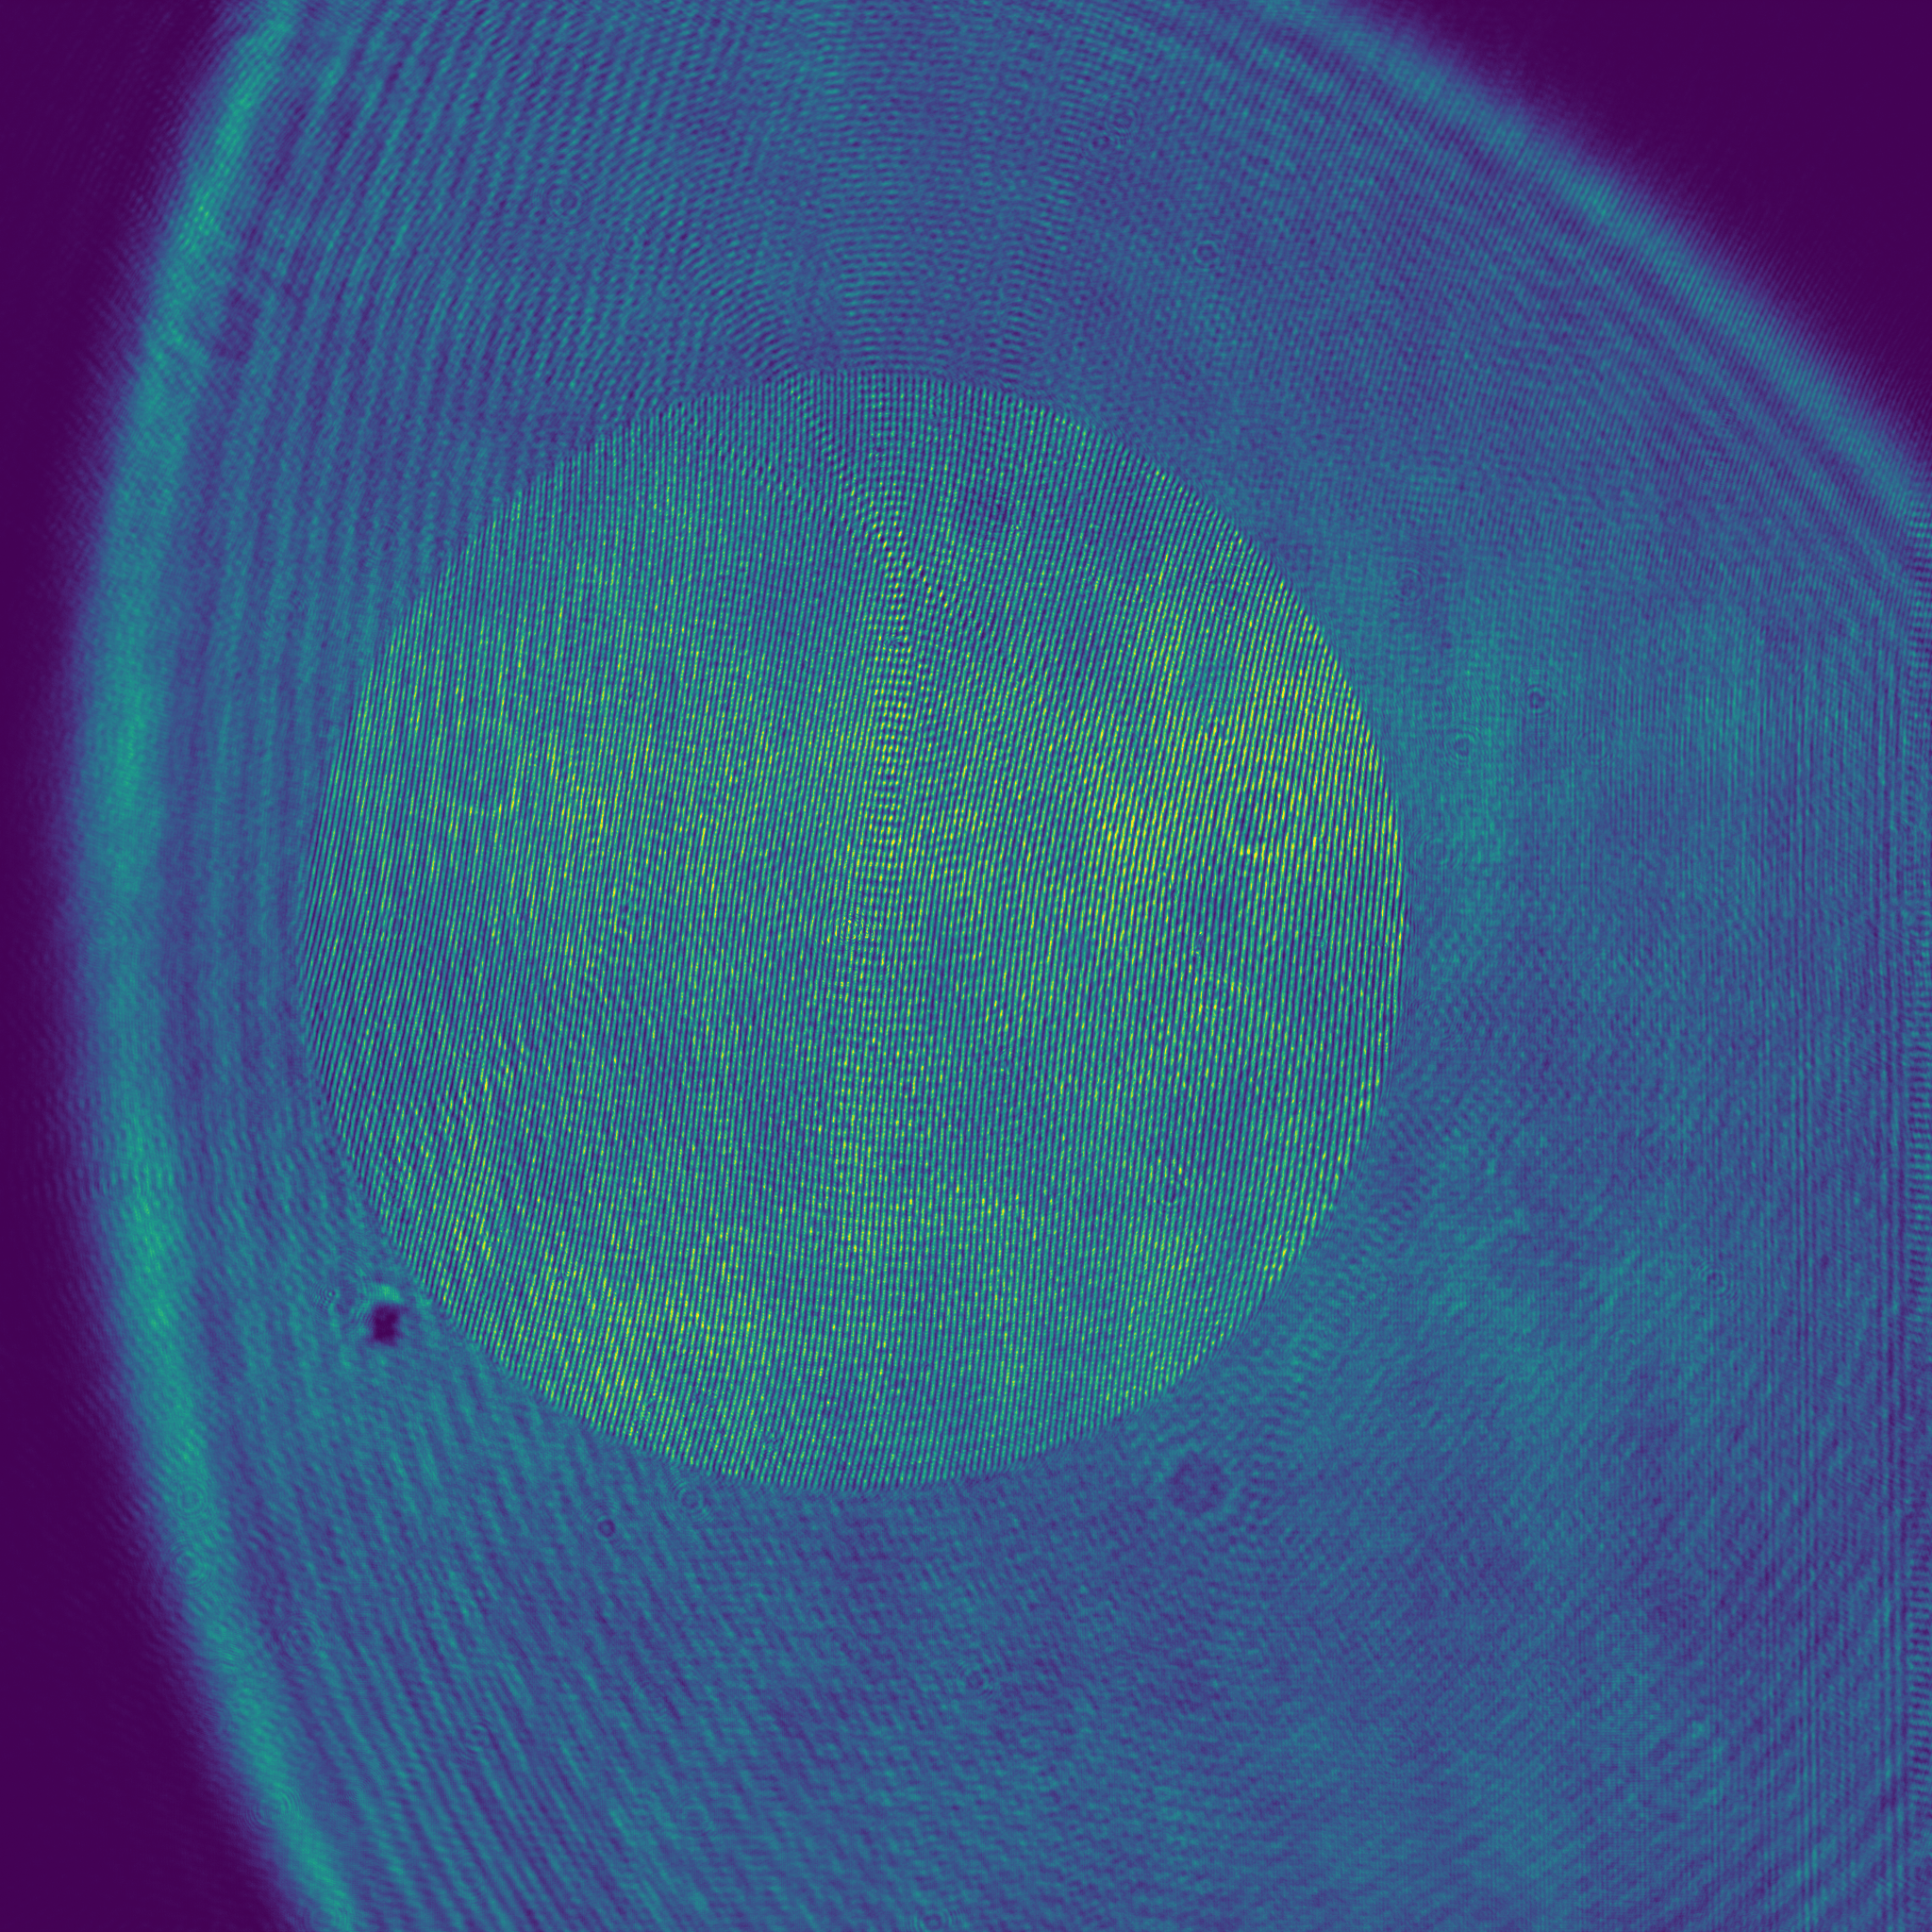
\includegraphics[width=1\linewidth, scale=0.5]{images/puw_inteferogram.png}
		\caption{}
		\label{fig:puw_inteferogram}
	\end{subfigure}
	\begin{subfigure}{0.23\textwidth}
		\centering
		\includegraphics[width=1\linewidth, scale=0.5]{images/puw_inteferogram_cropped.png}
		\caption{}
		\label{fig:puw_inteferogram_cropped}
	\end{subfigure}
	\begin{subfigure}{0.23\textwidth}
		\centering
		\includegraphics[width=1\linewidth, scale=0.5]{images/puw_mask.png}
		\caption{}
		\label{fig:puw_mask}
	\end{subfigure}
	\begin{subfigure}{0.23\textwidth}
		\centering
		\includegraphics[width=1\linewidth, scale=0.5]{images/puw_data_masked.png}
		\caption{}
		\label{fig:puw_data_masked}
	\end{subfigure}
	
	\begin{subfigure}{0.23\textwidth}
		\centering
		\includegraphics[width=1\linewidth, scale=0.5]{images/puw_data_fftshift.png}
		\caption{}
		\label{fig:puw_data_fftshift}
	\end{subfigure}
	\begin{subfigure}{0.23\textwidth}
		\centering
		\includegraphics[width=1\linewidth, scale=0.5]{images/puw_tukey_window.png}
		\caption{}
		\label{fig:puw_tukey_window}
	\end{subfigure}
	\begin{subfigure}{0.23\textwidth}
		\centering
		\includegraphics[width=1\linewidth, scale=0.5]{images/puw_fringes_tukey.png}
		\caption{}
		\label{fig:puw_fringes_tukey}
	\end{subfigure}
	\begin{subfigure}{0.23\textwidth}
		\centering
		\includegraphics[width=1\linewidth, scale=0.5]{images/puw_new_fringe_fft.png}
		\caption{}
		\label{fig:puw_new_fringe_fft}
	\end{subfigure}
	
	\begin{subfigure}{0.23\textwidth}
		\centering
		\includegraphics[width=1\linewidth, scale=0.5]{images/puw_new_fringe_fft_centre_blocked.png}
		\caption{}
		\label{fig:puw_new_fringe_fft_centre_blocked}
	\end{subfigure}
	\begin{subfigure}{0.23\textwidth}
		\centering
		\includegraphics[width=1\linewidth, scale=0.5]{images/puw_fft_filter.png}
		\caption{}
		\label{fig:puw_fft_filter}
	\end{subfigure}
	\begin{subfigure}{0.23\textwidth}
		\centering
		\includegraphics[width=1\linewidth, scale=0.5]{images/puw_new_fringe_order1.png}
		\caption{}
		\label{fig:puw_new_fringe_order1}
	\end{subfigure}
	\begin{subfigure}{0.23\textwidth}
		\centering
		\includegraphics[width=1\linewidth, scale=0.5]{images/puw_order1_roll.png}
		\caption{}
		\label{fig:puw_order1_roll}
	\end{subfigure}
	
	\begin{subfigure}{0.23\textwidth}
		\centering
		\includegraphics[width=1\linewidth, scale=0.5]{images/puw_complex_phase.png}
		\caption{}
		\label{fig:puw_complex_phase}
	\end{subfigure}
	\begin{subfigure}{0.23\textwidth}
		\centering
		\includegraphics[width=1\linewidth, scale=0.5]{images/puw_phaseorder1.png}
		\caption{}
		\label{fig:puw_phaseorder1}
	\end{subfigure}
	\begin{subfigure}{0.23\textwidth}
		\centering
		\includegraphics[width=1\linewidth, scale=0.5]{images/puw_phaseorder1mask}
		\caption{}
		\label{fig:puw_phaseorder1mask}
	\end{subfigure}
	\begin{subfigure}{0.23\textwidth}
		\centering
		\includegraphics[width=1\linewidth, scale=0.5]{images/puw_unwrapped_phase.png}
		\caption{}
		\label{fig:puw_unwrapped_phase}
	\end{subfigure}
	\caption[Visualisation of the stages of the phase acquisition workflow.]{Visualisation of the stages of the phase acquisition workflow. \textbf{(a)} Captured interferogram \textbf{(b)} Interferogram cropped to region of interest (ROI) \textbf{(c)} Circular mask \textbf{(d)} ROI isolated \textbf{(e)} ROI quadrant shifted (ROI-qs) \textbf{(f)} 2-D tukey window mask \textbf{(g)} ROI-qs with tukey mask applied \textbf{(h)} Fast Fourier transform (FFT) of \textbf{(g)}, log scaled \textbf{(i)} Fourier transform with the central spatial frequencies masked, log scaled \textbf{(j)} 2-D sine squared mask centred on the position of spatial frequencies encoding the phase information \textbf{(k)} The original Fourier transform, \textbf{(h)}, with the sine squared mask applied \textbf{(l)} Phase encoding spatial frequencies rolled to the central position \textbf{(m)} Inverse FFT of the phase encoding spatial frequencies \textbf{(n)} Inverse FFT transformed into a phase map \textbf{(o)} Phase map masked to isolate ROI \textbf{(p)} Phase map unwrapped to remove 2$\pi$ discontinuities}
	\label{fig:phase_unwrap_workflow}
\end{figure*}

Having performed the FFT (\ref{fig:puw_new_fringe_fft}), an array described by Equation~\ref{eq:I_fourier} is obtained. A selection of the central spatial frequencies are masked (\ref{fig:puw_new_fringe_fft_centre_blocked}), primarily to mask out the central spatial frequency which represents the mean intensity and has an amplitude orders of magnitude larger than any other spatial frequency. The spatial frequencies which now have the highest amplitudes correspond to both $\boldsymbol{C}(u,v)$ and $\boldsymbol{C}^{*}(u,v)$. One of the aforementioned amplitude peaks is located and a bandpass filter described by $\sin^{2}(x,y)$ is constructed (\ref{fig:puw_fft_filter}) centred on the spatial frequency location of this amplitude peak. As previously noted, the Fourier transform of the interferogram is symmetrical around the central spatial frequency. So, it doesn't matter which of the two peaks this filter is centred on since they encode the same information. The aforementioned bandpass filter is then applied to the FFT of the interferogram (\ref{fig:puw_new_fringe_order1}) and these spatial frequencies are then rolled to the central spatial frequency position (\ref{fig:puw_order1_roll}). Applying this successfully filters $\boldsymbol{A}(u,v)$ and $\boldsymbol{C}^{*}(u,v)$, isolating $\boldsymbol{C}(u,v)$ as desired.

The array corresponding to $\boldsymbol{C}(u,v)$ is inverse Fourier transformed to yield $c(x,y)$ (\ref{fig:puw_complex_phase}). This is then converted to a phase map by performing the calculation in Equation~\ref{eq:phase} (\ref{fig:puw_phaseorder1}) and the mask in Figure~\ref{fig:puw_mask} is applied again to mask out any spurious noise outside the ROI. Due to the periodic nature of trigonometric functions, this phase map is wrapped around $-\pi$ and $\pi$. An 2D  algorithm is used to unwrap the phase map and yield a phase Figure~\ref{fig:puw_unwrapped_phase} is obtained.\cite{herraez2002fast} Other than determining the appropriate ROI, this workflow is entirely automated and requires no user input. 

Automation does have a drawback. The location of the phase component of the Fourier transform is determined by finding the maximum intensity in the data represented by Figure~\ref{fig:puw_new_fringe_fft_centre_blocked} and then performing a number of centre of mass calculations to find the `true' centre of the phase component. However, this `true' centre may still be incorrect by a few pixels. This offset leads to an artificial introduction of tip and/or tilt in the final wavefront and this artificial tip/tilt cannot be separated from the true tip/tilt. Therefore, the described phase acquisition implementation cannot be said to be sensitive to tip or tilt. However, since tip and tilt (along with piston) are not considered to be a true optical aberration, this is a small price to pay for a fully automated phase acquisition workflow.

This phase extraction technique is used as part of other methods, but it is also useful for a user to be able to visualise the wavefront phase map. Principally this is because if the interferogram is not well focused on the camera it can result in the wavefront being heavily distorted by the Zernike mode corresponding to the defocus optical aberration (Noll Index 4). This can mask smaller wavefront deformations caused by the movement of the DM actuators and therefore bias calibration measurements. It can also be useful to view the system aberrations present, to check the difference applying the system aberration correction makes to the wavefront shape and to manually check for discontinuities. Cockpit implements such a method as the functionality of the "Visualise Phase" button shown in Figure~\ref{fig:DM_methods_cockpit}. This spawns the window shown in Figure~\ref{fig:phase_viewer_phase}, displaying the phase wavefront acquired from the interferogram. The display can be changed to the power spectrum of the interferogram, Figure~\ref{fig:phase_viewer_ft}, and back by pressing the "Real/Fourier Transform switch" button. 

\begin{figure}[h]
	\centering
	\begin{subfigure}{0.45\textwidth}
		\centering
		\includegraphics[width=1\linewidth, scale=0.5]{images/phase_viewer_phase.jpg}
		\caption{}
		\label{fig:phase_viewer_phase}
	\end{subfigure}
	\begin{subfigure}{0.45\textwidth}
		\centering
		\includegraphics[width=1\linewidth, scale=0.5]{images/phase_viewer_ft.jpg}
		\caption{}
		\label{fig:phase_viewer_ft}
	\end{subfigure}
	\caption[User interface for viewing the phase wavefront]{User interface for viewing the phase wavefront \textbf{(a)} Phase viewer window showing the unwrapped phase acquired from the interferogram \textbf{(b)} Phase viewer window showing the power spectrum of the interferogram. }
	\label{fig:phase_viewer}
\end{figure}

\subsection{Calibration}
\label{subsec:calibration}

For aberration correction, one could attempt to measure the overall aberration of the optical wavefront and apply the opposite shape to the DM. For direct wavefront sensing, this would appear as simple as measuring the phase distortion and shaping the DM to cancel this distortion. However, for continuous membrane DMs (which the majority of commercially available DMs are) the response of mirror shape to the actuators which control the mirror shape is generally non-linear, due to the membrane's mechanical elasticity, electrostatic forces and the coupling between actuators.\cite{Zhu:99} For indirect wavefront sensing this presents an even greater problem since any minimisation of the wavefront aberration would involve \textit{N} degrees of freedom, where \textit{N} is the number of actuators. Assuming that the overall mirror shape is the linear 
superposition of all the individual actuator deflections, we can 
define the overall mirror shape, $S(x,y)$ as:

\begin{equation}\label{eq:surface_shape}
S(x,y) = \sum_{h=1}^{N} d_{h}\phi_{h}(x,y)
\end{equation}

Where $S(x,y)$ is the change in the deformable mirror shape from its original position, $d_h$ is the $h$-th actuator control signal (an arbitrary value related to applied voltage which determines the position the $h$-th actuator in its overall movement range) and $\phi_{h}(x,y)$ is the $h$-th influence function. These are called the influence functions of the AO device since they describe how the elements of the device influence the phase wavefront. We can change this set of basis functions for a different basis set. An obvious alternative basis set is the Zernike polynomials since they are defined on the unit circle, orthogonal and the wavefront distortion can be well approximated by the linear addition of Zernike polynomials\cite{von1934beugungstheorie,noll1976zernike,mahajan1994zernike}. Describing $\phi_{h}(x,y)$ in terms of Zernike polynomials we obtain:

\begin{equation}\label{eq:influence_to_zernike}
\phi_{h}(x,y) = \sum_{g=1}^{M} b_{g,h}z_{g}(x,y)
\end{equation}

Where $b_{g,h}$ is the coefficient corresponding to the $k$-th Zernike polynomial due to the $d_h$. The change in mirror shape, $\Delta S(x,y)$, can therefore be described as:

\begin{equation}\label{eq:zernike_sub}
\begin{split}
\Delta S(x,y) & = \sum_{h=1}^{N} d_{h}\left[\sum_{g=1}^{M} b_{g,h}z_{g}(x,y)\right] \\
& =\sum_{g=1}^{M} \left(\sum_{h=1}^{N} d_{h} b_{g,h}\right) z_{g}(x,y) \\
& =\sum_{g=1}^{M} a_{g} z_{g}(x,y)
\end{split}
\end{equation}

Where the new Zernike coefficients, $a_{g}$, is defined as:

\begin{equation}\label{eq:new_z_coef}
a_{g} = \sum_{h=1}^{N} b_{g,h} d_{h} \text{~for~} g=1,2,...,M
\end{equation}

Converting Equation~\ref{eq:new_z_coef} to a matrix form yields:

\begin{equation}\label{eq:CM_derivation}
\begin{split}
\bar{a} &= \boldsymbol{B} \bar{d}\\
\Rightarrow \bar{d} &= \boldsymbol{C} \bar{a}
\end{split}
\end{equation}

Where $\bar{d}$ is a length $N$ vector of the actuator control signals, $\bar{a}$ is the length $M$ vector of the Zernike polynomial amplitudes and $\boldsymbol{B}$ is the $M \times N$ matrix representing the response characteristics of the deformable mirror. However, we actually want its inverse, $\boldsymbol{B}^{-1} =\boldsymbol{C}$, otherwise called the control matrix in order to convert from Zernike polynomial amplitudes to actuator control signals.

Microscope-AOtools implements an automated calibration routine to obtain $\boldsymbol{C}$. Each actuator is moved through $p$ set positions and a wavefront is extracted. Figure~\ref{fig:observed_wavefront} shows an observed wavefront during the calibration routine. The wavefront is then decomposed into $M$ Zernike modes\cite{townson2019aotools}. A row vector $\boldsymbol{z}$ is obtained for each actuator position containing the computed Zernike mode amplitudes:

\begin{equation}\label{eq:zernike_amp}
\boldsymbol{z} = 
\begin{bmatrix}
z_{1} & z_{2} & \cdots & z_{m} 
\end{bmatrix}
\end{equation}

Where the $g$-th element is the amplitude of the $g$-th
Zernike mode. Figure~\ref{fig:measured_zernike_modes} shows
a plot of the row vector containing the amplitudes of the 
$M$ Zernike modes measured for Figure~\ref{fig:observed_wavefront}.
Figure~\ref{fig:simulated_wavefront} show a simulated wavefront 
constructed using these Zernike mode amplitudes. As previously 
mentioned, a phase wavefront can be constructed from an 
infinite linear combination of Zernike modes\cite{noll1976zernike}. 
However, using a finite number of Zernike modes produces only an 
approximation of the original wavefront. 
Figure~\ref{fig:observed_simulated_wavefront_diff} show the
difference between the two and a ``ringing'' analogous to the 
Gibbs phenomena for recreating periodic signals using a
truncated Fourier series is present.

By collecting the row vectors of each position
for the $h$-th actuator we can obtain:

\begin{equation}\label{eq:zernike_amp_actuator}
A_h = 
\begin{bmatrix}
\boldsymbol{z_{1}}\\
\boldsymbol{z_{2}}\\
\vdots\\
\boldsymbol{z_{p}} 
\end{bmatrix}
=
\begin{bmatrix}
z_{1,1} & z_{1,2} & \cdots & z_{1,m} \\
z_{2,1} & z_{2,2} & \cdots & z_{2,m} \\
\vdots  & \vdots  & \ddots & \vdots  \\
z_{p,1} & z_{p,2} & \cdots & z_{p,m} 
\end{bmatrix}
\end{equation}

Linear regression to each column, $\begin{bmatrix} z_{1,i} & z_{2,i} & \cdots & z_{p,i} \end{bmatrix}^T$, yields the response characteristics between the $h$-th actuator's position and the $g$-th Zernike mode, $b_{g,h}$. Figure~\ref{fig:influence_function_11} shows the influence function fitting for Zernike mode 11 (Noll index) for the $26^{th}$ actuator. The gradient of the slope is, in this case, $b_{11,26}$. This gradient is acquired for each actuator, for each Zernike mode. In this way, we construct $\boldsymbol{B}$ and then calculate $\boldsymbol{C}$. Figure~\ref{fig:calibration_workflow} shows a flowchart of this process as implemented in Microscope-AOtools.

\begin{figure}[h]
	\centering
	\begin{subfigure}{0.285\textwidth}
		\centering
		\includegraphics[width=1\linewidth, scale=0.5]{images/observed_wavefront.png}
		%\caption{Observed wavefront}
		\caption{}
		\label{fig:observed_wavefront}
	\end{subfigure}
	\begin{subfigure}{0.285\textwidth}
		\centering
		\includegraphics[width=1\linewidth, scale=0.5]{images/simulated_wavefront.png}
		%\caption{Simulated wavefront}
		\caption{}
		\label{fig:simulated_wavefront}
	\end{subfigure}
	\begin{subfigure}{0.345\textwidth}
		\vspace{-0.2cm}
		\centering
		\includegraphics[width=1\linewidth, scale=0.5]{images/observed_simulated_wavefront_diff.png}
		%\caption{Difference between observed and simulated wavefront}
		\caption{}
		\label{fig:observed_simulated_wavefront_diff}
	\end{subfigure}
	
	\begin{subfigure}{0.45\textwidth}
		\centering
		\includegraphics[width=1\linewidth, scale=0.5]{images/measured_zernike_modes.png}
		%\caption{Zernike mode amplitudes measured in the observed wavefront}
		\caption{}
		\label{fig:measured_zernike_modes}
	\end{subfigure}
	\begin{subfigure}{0.45\textwidth}
		\centering
		\includegraphics[width=1\linewidth, scale=0.5]{images/influence_function_11.png}
		%\caption{Influence function fitting}
		\caption{}		
		\label{fig:influence_function_11}
	\end{subfigure}
	\caption[Visualisation of the influence function fitting stage of the calibration routine]{Visualisation of the influence function fitting stage of the calibration routine \textbf{(a)} An example observed wavefront obtained during the calibration process for an Alpao-69 actuator deformable mirror. The $26^{th}$ actuator is at the first of the 5 positions. \textbf{(b)} A simulated wavefront created from the 69 Zernike mode amplitudes measured in the observed wavefront. \textbf{(c)} The difference in the observed and simulated wavefronts. \textbf{(d)} The 69 Zernike mode amplitudes measured for the observed wavefront \textbf{(e)} The influence function fitting for Zernike mode 11 (Noll index) for the $26^{th}$ actuator}
	\label{fig:wavefront_decomposition}
\end{figure}

\begin{figure}[h]
	\centering
	\begin{subfigure}{0.45\textwidth}
		\centering
		\includegraphics[width=1\linewidth, scale=0.5]{images/calibration_routine_workflow.jpg}
		\caption{}
		\label{fig:calibration_routine_workflow}
	\end{subfigure}
	\begin{subfigure}{0.45\textwidth}
		\centering
		\includegraphics[width=1\linewidth, scale=0.5]{images/Ith_actuator_calibration_workflow_blue_border.jpg}
		\caption{}
		\label{fig:Ith_actuator_calibration_workflow_blue_border}
	\end{subfigure}
	\caption[Calibration routine workflow]{\textbf{(a)} Flowchart depicting the generalised calibration routine implemented in Mircoscope-AOtools \textbf{(b)} Flowchart depicting the the process for calibrating the $h$-th actuator of the deformable mirror, the dashed blue process in \textbf{(a)}. The influence functions returned are $b_{g,h}$ described in Equation~\ref{eq:influence_to_zernike}. This process is performed for each $N$ actuators and used to obtain $\boldsymbol{C}$ described in Equation~\ref{eq:CM_derivation}.}
	\label{fig:calibration_workflow}
\end{figure}

In general, $\boldsymbol{B}$ is singular and therefore has no true inverse and so we must use a pseudo-inverse, calculated using single value decomposition (SVD). However, some values of $\boldsymbol{B}$ may be small since the physical position of certain actuators will mean they have limited influence on creating certain Zernike modes. A control matrix calculated without thresholding out these small values will quickly lead to a saturation of the DM actuators (i.e. all actuators at their maximum stroke length) when corrections are calculated.\cite{booth2005methods} Therefore the calibration method incorporates a threshold by default and the exact threshold can be varied by experienced users. The calibration routine is initiated by pressing the "Calibrate" button shown in Figure~\ref{fig:DM_methods_cockpit}.

\subsection{Characterisation}
\label{subsec:characterisation}

Feedback on the quality of the calibration process is essential. Ideally, once the deformable mirror is calibrated we have a linear map which allows known quantities of Zernike modes to be applied exactly. This linear map is never exact in practice due to issues; the fact that some parameters, such as the number of steps used to calibrate each actuator and the threshold used in the SVD pseudo-inversion, are chosen empirically, the approximate nature of the pseudo-inverse, discretisation errors (due to discrete sampling of a continuous functions) in the measuring of Zernike modes. etc It is therefore necessary to have some measure of how well the adaptive element is able to recreate desired Zernike modes. This process is called characterisation. The process involves applying a fixed amplitude of single Zernike modes to the adaptive element, measuring the Zernike modes present and comparing the amplitude to that supposedly applied. An automated implementation of this process is present in Microscope-AOtools with the results returned to the user for interrogation. Figure~\ref{fig:characterisation_workflow} shows a flowchart of this method in Microscope-AOtools. 

\begin{figure}[h]
	\centering
	\includegraphics[width=0.4\textwidth, scale=0.5]{./images/characterisation_workflow.jpg}
	\caption[Characterisation routine workflow]{Flowchart depicting the process for characterising a deformable mirror as implemented in Microscope-AOtools}
	\label{fig:characterisation_workflow}
\end{figure}

In an ideal situation, where the control matrix provided a perfect linear map from Zernike mode amplitudes to the adaptive elements degrees of freedom, a characterisation assay like Figure~\ref{fig:characterisation_assay_ideal} is expected, where only the Zernike mode applied is measured. In practice, the adaptive element is better at recreating particular Zernike modes and some Zernike mode coupling is observed i.e. Zernike modes which were not applied to the adaptive element are measured. This leads to characterisation assays like Figure~\ref{fig:characterisation_assay_real}. Here we present a characterisation assay obtained for an Alpao-69 actuator deformable mirror. We define a recreation accuracy metric, $\alpha_{i}$, for each mode:

\begin{equation}\label{eq:recreation_accuracy}
\begin{split}
\alpha_{i} &= \frac{Z'_{i} - \boldsymbol{RMS}(Z'_{j})}{Z_{i}} \\
&= \frac{Z'_{i} - \sqrt{\frac{1}{N-1}\sum_{j=0,j\ne i}^{N} {Z'_{j}}^{2}}}{Z_{i}}
\end{split}
\end{equation}

Where $Z_{i}$ is the applied Zernike mode amplitude, $Z'_{i}$ and $Z'_{j}$ are the measured Zernike mode amplitudes for the current mode and all other modes respectively and $N$ is the number of Zernike modes being assessed. Figure~\ref{fig:real_characterisation_assay_plot_metric_errorbar} shows a plot of this metric for the characterisation assay in Figure~\ref{fig:characterisation_assay_real}. The errorbars are determined by the standard deviation of $\boldsymbol{RMS}(Z'_{j})$

\begin{figure}[h]
	\centering
	\begin{subfigure}{0.45\textwidth}
		\centering
		\includegraphics[width=0.8\linewidth, scale=0.5]{./images/characterisation_assay_ideal.png}
		\caption{}
		\label{fig:characterisation_assay_ideal}
	\end{subfigure}
	\begin{subfigure}{0.45\textwidth}
		\centering
		\includegraphics[width=1\linewidth, scale=0.5]{./images/characterisation_assay_real.png}
		\caption{}
		\label{fig:characterisation_assay_real}
	\end{subfigure}
	\begin{subfigure}{0.9\textwidth}
		\centering
		\includegraphics[width=0.6\linewidth, scale=0.5]{./images/real_characterisation_assay_plot_metric_errorbar.png}
		\caption{}
		\label{fig:real_characterisation_assay_plot_metric_errorbar}
	\end{subfigure}
	\caption[Example characterisation routine results]{Example characterisation routine results \textbf{(a)} An ideal characterisation assay, measuring the recreation accuracy of 68 Zernike modes with applied amplitude of 1 for each \textbf{(b)} A realistic characterisation assay obtained from a calibrated Alpao-69 actuator deformable mirror, measuring the recreation accuracy of 68 Zernike modes with applied amplitude of 1 for each \textbf{(c)} Plot of the recreation accuracy metric for the real characterisation assay shown in \textbf{(b)}. The threshold (red dashed line) is set at 0.75}
	\label{fig:characterisation_assay_results}
\end{figure}

Clearly not all Zernike modes are recreated equally well and  different modes exhibit varying degrees of mode coupling. As previously mentioned, this arises from mathematical approximations,
computational errors and the physical characteristics of the adaptive element. Microscope-AOtools provides the tools to assess the accuracy of Zernike mode recreation, which can be used to inform which modes should be included in the aberration correction algorithms.

The characterisation routine relies on the same generalised phase acquisition method used in the calibration workflow. Recall that this is a user selected method from a suite of phase acquisition methods. The number of Zernike modes assessed, $N$, is the number of modes that have been measured in the calibration step by default, but this can be varied by the user. Once again this preserves generalisability and allows the characterisation method to be used on any arbitrary adaptive element, calibrated for any number of modes and utilising any desired wavefront sensing technique.

\subsection{System Aberration Correction}
\label{subsec:system_correction}

The applications for aberration correction using direct wavefront sensing have been well documented. The wavefront is measured via interferometry, Shack-Hartmann wavefront sensor, fluorescent guide star, etc and decomposed into Zernike modes. Correction can then be calculated and applied for both system and sample induced aberrations. Microscope-AOtools implements a correction method for situations where the wavefront is directly observed. The workflow is shown in Figure~\ref{fig:direct_wavefront_flattening_workflow}. The wavefront is obtained through whatever direct wavefront sensing method has been implemented and selected, a number of Zernike modes determined by the user are fitted to the wavefront, an equal and opposite magnitude of these modes are applied to the DM. The RMS wavefront error is then calculated. This process repeats until $N$ iterations have been performed or the RMS wavefront error is below a user defined error threshold, $\delta$.

\begin{figure}[h]
	\centering
	\includegraphics[width=0.55\textwidth, scale=0.5]{./images/direct_wavefront_flattening_workflow.jpg}
	\caption[Direct wavefront correction workflow]{Flowchart depicting the process for flattening directly measured wavefront as implemented in Microscope-AOtools}
	\label{fig:direct_wavefront_flattening_workflow}
\end{figure}

In an ideal setup with a perfect control matrix, this process would only need to be performed once. However, as we have already discussed, the control matrices generated for any setup are never ideal due to non-linearities and inter-actuator coupling. Therefore, one iteration of this method would correct the aberrations to an extent, but it would leave residual aberrations. It is necessary to perform this process for a number of iterations to ensure the optimal wavefront is obtained. 

Figure~\ref{fig:direct_wavefront_correction} shows the results of one such wavefront correction, performed using the same Alpao-69 actuator deformable mirror as shown in Figure~\ref{fig:DeepSIM_complete_beam_paths}. The wavefront was 
obtained by interferometry and Zernike modes 5-29 (using Noll indices) were corrected over 20 iterations. The RMS phase errors in Figures~\ref{fig:aberrated_wavefront_defocus_ptt_rmv_crop_phase_only} and \ref{fig:flattened_wavefront_20it} are 3.818 radians and 0.986 radians of 543nm respectively. A significant portion of the phase deformation after correction seems to be located at the edges of the aperture. The RMS phase error of the central 95\% of the phase wavefront is 0.712 radians, equivalent of a Strehl ratio $\approx 0.602$. Figure~\ref{fig:zernike_modes_to_show_flattening}
shows the Zernike mode amplitudes before and after correction. The dots visible are the physical location of the actuators on the deformable mirror and represent a limiting factor in how flat the deformable mirror surface can actually be. 

\begin{figure}[h]
	\centering
	\begin{subfigure}{0.4\textwidth}
		\centering
		\includegraphics[width=1\linewidth, scale=2]{./images/system_wavefront_before_correction_adv.png}
		\caption{}
		\label{fig:aberrated_wavefront_defocus_ptt_rmv_crop_phase_only}
	\end{subfigure}
	\begin{subfigure}{0.49\textwidth}
		\centering
		\vspace{-.25cm}
		\includegraphics[width=1\linewidth, scale=2]{./images/system_wavefront_after_correction_best_20it_adv.png}
		\caption{}
		\label{fig:flattened_wavefront_20it}
	\end{subfigure}
	
	\begin{subfigure}{0.55\textwidth}
		\centering
		\includegraphics[width=1\linewidth, scale=1]{./images/Zernike_modes_before_after_correction_only_corrected.png}
		\caption{}
		\label{fig:zernike_modes_to_show_flattening}
	\end{subfigure}
	\caption[Example direct wavefront correction results]{Example direct wavefront correction results \textbf{(a)} An aberrated wavefront \textbf{(b)} A wavefront after 20 iterations of correction \textbf{(c)} The Zernike mode amplitudes measured in the aberrated (red) and corrected (blue) wavefronts \textbf{(a)} - \textbf{(b)} are all presented on the same colorscale (in radians of 543nm HeNe laser) and were obtains via interferometry}
	\label{fig:direct_wavefront_correction}
\end{figure}

For system aberration corrections it may be preferable to set a minimum wavefront error and continue to iterate until this threshold is reached. However a user may wish to only spend $N$ iterations correcting the wavefront. Microscope-AOtools implements both options to ensure generalisability and these parameters can be set by the user utilising the option window shown in Figure~\ref{fig:DM_direct_wavefront_sensing_options}. As with the calibration and characterisation methods, the wavefront flattening routine relies on a user selected phase acquisition method selected from the suite of implemented phase acquisition methods. This generalised construction ensures that the applicability of Microscope-AOtools to any adaptive element with any wavefront sensing technique is preserved throughout all the set-up methods.

The characterisation routine is initiated by pressing the "Calculate System Flat" button shown in Figure~\ref{fig:DM_methods_cockpit}. Spawning the window shown in Figure~\ref{fig:DM_direct_wavefront_sensing_options} allows a user to vary the number of iterations and RMS error threshold used for the wavefront correction routine. By default the routine runs for exactly 10 iterations, since the default error threshold is $\infty$ and so any wavefront deformation will yield an RMS value under this threshold. A user can also vary the Zernike modes the wavefront flatting routine will try to correct for. By default the Zernike modes corrected for are all Zernike modes with Noll indices, $j$, $\ge$ 4 (i.e. all the true optical aberrations) and $<$ the number of actuators, N. Once the Characterisation routine has been performed this is changed to be all Zernikes modes with $4 \le j < N$ and with a recreation accuracy within 1 standard deviation of 0.75.  Once the actuator values for correcting the system aberrations have been calculated they are stored in Cockpit's internal configuration and can be applied at any time using the "System Flat" button shown in Figure~\ref{fig:DM_methods_cockpit}.

\section{Sample Correction Methods}
\label{sec:sample_correction_methods}

\subsection{Sensorless Correction}
\label{subsec:sensorless_correction}

In many biological applications, direct wavefront sensing is not possible and so we rely on sensorless techniques to determine the best correction to apply. The generalised methodology for this is shown in Figure~\ref{fig:sensorless_correction_method}. Some metric, $S$, which gives a useful measure of the image quality is chosen. This metric should be a numerical value and should 
increase to a global maximum as the aberrations present decrease. Often these metrics are related to common measures of image quality, such as sharpness or contrast. For each Zernike mode, $Z_{i}$, a number of amplitudes of that mode, $a_{j}$, are applied and an image of the sample obtained. The quality of each image, $S_{j}$ is calculated. Assuming that $S$ is a function of the Zernike mode amplitude applied,	fitting a Gaussian function to the $S_{j}$ values yields a Zernike mode amplitude, $a_{max}$, which theoretically yields the best image quality, $S_{max}$. The complexity of sensorless AO correction lies in selecting the most appropriate image quality metric. There 
have been numerous metrics developed which have been shown to be effective on certain sample types or imaging modalities\cite{burke2015adaptive,booth2002adaptive,fienup2003aberration,debarre2008adaptive}.

\begin{figure}[h]
	\centering
	\includegraphics[width=1\textwidth,scale=0.5]{./images/sensorless_aberration_fitting_w_images.png}
	\caption[Principle of sensorless adaptive optics correction.]{Principle of sensorless adaptive optics correction. For each Zernike mode, $Z_i$, images of the sample with different amplitudes of the $i$-th Zernike mode are obtained. A value of the image quality metric, $S$, is obtained for each (blue dots). A Gaussian function is then fitted to these image quality metric values and the amplitude, $a$ corresponding to the maximum image quality, $S_{max}$, is obtained (green dot). The inset images are Drosophila Neuro-muscular Junction with various amplitudes of spherical aberration present.}
	\label{fig:sensorless_correction_method}
\end{figure}

The complexity of sensorless adaptive optics correction lies in selecting the best image quality metric. There have been numerous metrics developed which have been shown to be effective on certain sample types or imaging modalities.\cite{burke2015adaptive,booth2002adaptive,fienup2003aberration,debarre2008adaptive} In order for an adaptive optics implementation to be considered generalised, it should not be tied to a particular sample type or imaging modality. For this reason, Microscope-AOtools offers a range of image quality metrics, all located in the \textit{aoMetrics.py}.  

Unlike the calibration, characterisation and direct wavefront sensing techniques, the sensorless adaptive optics routine is not a method implemented in Microscope-AOtools and simply called by Cockpit. Instead, the sensorless correction routine relies on coordination between Cockpit, Python Microscope and Microscope-AOtools. The biological sample is set up in the image plane. A known amplitude of the first Zernike mode to be corrected for is applied to the DM by Microscope-AOtools, Then the light sources and camera are triggered by Python Microscope and the image data is collected by Cockpit. This is repeated for $M$ measurements. Then, Cockpit passes the $M$ images to Microscope-AOtools where the image quality metric for each image is evaluated. These values are then used to fit a Gaussian function and the mean of the Gaussian yields the Zernike mode amplitudes which should yield the maximum image quality, $a_{max}$. This amplitude is then applied to the DM and stored as the offset on top of which all further corrections should be applied. This process is then repeated for $N$ Zernike modes. This whole process is further repeated for $T$ iterations. Finally, the recorded Zernike mode amplitudes which have been corrected for and the actuator positions associated with that correction are stored in in Cockpit's internal configuration. The sensorless adaptive optics routine is initiated by pressing the "Sensorless AO" button shown in Figure~\ref{fig:DM_methods_cockpit}. The workflow of this routine is shown in Figure~\ref{fig:sensorless_correction_workflow_DeepSIM}

\begin{figure}[h]
	\centering
	\includegraphics[scale=0.65]{./images/sensorless_correction_workflow_DeepSIM.jpg}
	\caption[Sensorless adaptive optics correction workflow]{Flowchart depicting the sensorless correction routine implemented on DeepSIM. All $M$ images are taken, then the quality metric is obtained for all $M$ images, the best Zernike amplitude is found and applied }
	\label{fig:sensorless_correction_workflow_DeepSIM}
\end{figure}

Clearly, this sensorless routine has multiple parameters and there is a limited degree to which these can be automatically selected. To this end, Figures~\ref{fig:DeepSIM_control_software} \&~\ref{fig:DM_methods_cockpit_options} allow the user to vary these parameters. Figure~\ref{fig:DM_methods_cockpit_options} shows various options the user can select for the image quality metric to be used. As previously mentioned, different image quality metrics are optimised for different imaging modalities and sample types. Allowing the user to easily switch between metrics is critical for a generalised implementation of adaptive optics which is accessible to non-experts. Figure~\ref{fig:DeepSIM_control_software} shows a window which allows the user to vary the number of iterations, $T$, the Zernike modes to be corrected, $N$ and the number of measurements for each mode, $M$. By default, the Zernike modes corrected for are $1^{st}$ and $2^{nd}$ order spherical aberration, coma, astigmatism and trefoil (in that order) as in biological samples these are often the source of the most significant wavefront deformation, and therefore loss of image quality. The amplitudes applied to the DM are evenly spaced between the "Aberration range minima", $j_{min}$ and "Aberration range maxima", $j_{max}$, in $M$ intervals. These are user specified variable, set using the window show in Figure~\ref{fig:DM_sensorless_ao_parameters}. 

The values for $j_{min}$ and $j_{max}$ should ideally be chosen to scan a sufficient range of aberration amplitudes to ensure $j_{min} \le a_{max} \le j_{max}$. At the least $a_{max}$ should be sufficiently close to $j_{min}$ or $j_{max}$ so that there is a clear increase in image quality as the aberration amplitude applied approaches one of these bounds. This range should not be too large otherwise a user risks either having sparse image quality data which only captures extreme aberrations and prevents an adequate fitting, or taking a sufficient number of measurements but introducing considerable photodamage. Like the image quality metrics, the $[j_{min},j_{max}]$ range will vary with sample type and so some preliminary work is required before data collection proper to ascertain the correct range as well as the correct number of measurements and iterations, $N$ and $T$, for a given sample type. 

As previously mentioned, the $[j_{min},j_{max}]$ range should ideally contain $a_{max}$ or $a_{max}$ should be close to one of these bounds. Allowing the Gaussian function to be fitted to the image quality metric values with no bounds (i.e. allowing $a_{max}$ to take any value) becomes problematic when the image quality metric values remain largely constant over all the amplitudes applied. This phenomenon can occur for a number of reasons; $a_{max}$ is found far outside the range of amplitudes scanned, the amplitudes sampled were sufficiently sparse that the central region of the Gaussian lies between two amplitudes, the aberration being sampled does not have a strong impact on the image quality measured, another, more significant aberration mode has not been corrected and the effect of this other mode is masking the effect of the current mode, etc. Whatever the reason, an unbounded fitting to a relatively flat profile of image quality metric measurements will lead to a large value of $a_{max}$ which is unreliable and often results in an applying an aberration amplitude which severly damages the image quality. To ensure that the Gaussian fitting to find $a_{max}$ yields a reasonable value, the fitting has bounds defined as $(j_{max}-j_{min}) \pm 0.25(j_{max}-j_{min})$.

\subsection{Image Quality Metric: Fourier Power}
\label{subsec:fourier_power_metric}

As mentioned in Section~\ref{subsec:sensorless_correction}, 
sensorless AO correction requires an image quality metric which
is well suited to both the imaging modality and the desired 
sample. Microscope-AOtools implements a suite of image quality
metrics to choose from. Both the DeepSIM and the Aurox
Clarity systems can be considered structured illumination
system. Although the Aurox Clarity system is clearly not a 
Gustafsson-style SIM system, the illumination pattern imposed by
the spinning disk. If follow that the image quality of both systems is
contingent on high quality Fourier information. Therefore, 
a sensible starting point for the image quality metric, $S$, 
is the total power of the Fourier spectrum:

\begin{equation}\label{eq:fourier_power_spectrum}
S = \sum\limits_{n,m}{\left\| \tilde{\textbf{D}}_{n,m} \right\|^2}
\end{equation}

Where $\tilde{\textbf{D}}$ is the 2D discrete Fourier transform of 
the fluorescent signal (i.e. the camera image) and $n$ and 
$m$ are the pixel coordinates with ranges $[0, N-1]$ and $[0, M-1]$ 
respectively, where $N$ and $M$ are the number of pixels along each 
dimension of the image. From Parseval's Theorem, $\sum\limits_{n,m}
\left\| \tilde{\textbf{D}}_{n,m} \right\|^2$ is the power of the 
observed signal. However, the Fourier spectrum obtained is not 
entirely composed of sample information. Recall that the fluorescent 
signal for a single image is the convolution of the distribution of 
fluorescent emission and the system point spread function (PSF):

\begin{equation}
\begin{split}
F(\textbf{r}) &= (E \circledast H)(\textbf{r})\\
F(\textbf{r}) &= [D(\bar{x})I(\textbf{r})] \circledast H(\textbf{r}),\\
\end{split}\tag{\ref{eq:fluorescent_image}}
\end{equation}

Where $D(\textbf{r})$ is the sample fluorescence distribution, 
$I(\textbf{r})$ is the illumination pattern, $E(\bar{x})$ is
the resultant emission signal and $H(\textbf{r})$ is the system 
point spread function (PSF). For a widefield image, 
$I(\textbf{r}) = 1$. Applying this substitution and a Fourier 
transform yields:

\begin{equation}\label{eq:fluor_signal_fourier}
\begin{split}
\mathcal{F}[\textbf{F}(\textbf{r})] &= \mathcal{F}[\textbf{D}(\textbf{r}) \circledast \textbf{H}(\textbf{r})]\\
\tilde{\textbf{F}}(\textbf{k}) &= \tilde{\textbf{D}}(\textbf{k}) \tilde{\textbf{H}}(\textbf{k})\\
&= \tilde{\textbf{D}}(\textbf{k}) \textbf{O}(\textbf{k})		
\end{split}
\end{equation}

Where the tilde ($\sim$) represent the Fourier transform of the corresponding 
real-space functions and $\textbf{O}(\textbf{k})$ is the system optical transfer 
function (OTF).\cite{gustafsson2008three} The OTF both attenuates the sample 
fluorescence distribution spatial frequencies and acts as a lowpass filter. 
Since $\tilde{\textbf{D}}_{n,m}$ is the 2D discrete Fourier transform of 
the observed data, this lowpass filter, $\mu_{n,m}$, is defined as:

\begin{equation}\label{eq:circular_mask}
\mu_{n,m} = 
\begin{cases}
1, & \sqrt{n'^{2} + m'^{2}} \le \omega_{l}\\
0, & \sqrt{n'^{2} + m'^{2}} > \omega_{l}\\ 
\end{cases}
\end{equation}

Where $n' = n - \frac{N-1}{2}$, $m' = m - \frac{M-1}{2}$ and $\omega_{l}$ 
is the lateral diffraction limit in reciprocal space as per
 Equation~\ref{eq:lateral_spatial_freq_res} 

Within the OTF lowpass limit, certain spatial frequencies will be dominated
by noise contributions. As such, when attempting to quantify the power 
contribution from the fluorescent it is desirable to ignore the noise
contributions. A thresholding mask, $\tau_{n,m}$ is created and defined as:

\begin{equation}\label{eq:noise_threshold_mask}
\tau_{n,m} = 
\begin{cases}
0, & \left\| \tilde{\textbf{D}}_{n,m} \right\|^2 < \delta\\
1, & \left\| \tilde{\textbf{D}}_{n,m} \right\|^2 \ge \delta\\ 
\end{cases}
\end{equation}

Where $\delta$ is a noise threshold defined as:

\begin{equation}\label{eq:noise_threshold}
\delta = \frac{\alpha}{P_{noise}}\sum\limits_{l,k}{\left\| \tilde{\textbf{D}}_{l,k} \right\|^2}
\end{equation}

Where $\left\| \tilde{\textbf{D}}_{l,k} \right\|^2$ is the power in the 
$l$-th, $k$-th spatial frequency where $l$ \& $k$ are the coordinates 
where $\mu_{n,m} = 0$, $P_{noise}$ is the total number of pixels 
outside the OTF lowpass limit and $\alpha$ is a user defined 
amplification factor. In essence, the threshold is the mean of the
power of the spatial frequencies consisting entirely of noise signals,
scaled by $\alpha$.	The value of $\alpha$ must be chosen to threshold
the spatial frequencies dominated by noise without losing the sensitivity
to true, albeit low amplitude, spatial frequencies. Empirically, an 
$\alpha = 1.125$ offers a reasonable compromise between these traits.

Finally, the bulk of the improvement in spatial frequency content will
occur in the mid to high frequencies (relative to $\omega_{l}$). As such there is 
a desire for increased sensitivity to the power fluctuations in these 
spatial frequencies. A modulation mask, $\omega$, is constructed and 
defined as:

\begin{equation}\label{eq:attenuation_mask_norm_and_scaled}
\omega_{n,m} = \beta \left| \left(1 - e^{\frac{\sqrt{n'^{2} + m'^{2}}}{\omega_{l}}-1}\right) \left(n'^{2} + m'^{2}\right) \right|
\end{equation}

Where $\omega_{l}$, $n'$ and $m'$ are defined as before, $\left|...\right|$ 
is $...$ normalised to $[0,1]$, and $\beta$ is a user defined 
normalisation factor. In effect, this modulation mask amplifies the mid 
to high spatial frequencies while attenuating the low spatial frequencies 
and the high spatial frequency noise close to $\omega_{l}$.

Applying these modification to Equation~\ref{eq:fourier_power_spectrum} 
yields the image quality metric:

\begin{equation}\label{eq:Fourier_power_metric}
S = \sum\limits_{n,m}{\mu_{n,m}\tau_{n,m}\omega_{n,m}\left\| \tilde{\textbf{D}}_{n,m} \right\|^2}
\end{equation}

Where $\mu_{n,m}$, $\tau_{n,m}$ and $\omega_{n,m}$ are defined as in
Equations~\ref{eq:circular_mask},~\ref{eq:noise_threshold_mask} and
\ref{eq:attenuation_mask_norm_and_scaled} respectively and 
$\tilde{\textbf{D}}_{n,m}$ is defined as before. In practice, $S$
measures the total power of the sample spatial frequencies, with 
increased sensitivity to mid to high spatial frequency changes. As
such, this image quality metric is called the Fourier Power metric.
As previously mentioned, SIM imaging depends on high quality spatial 
frequency information.\cite{debarre2008adaptive,thomas2015enhanced} 
Since the Fourier Power imaging metric maximises the intensity of 
the mid-high spatial frequency content, this image quality metric 
is particularly well suited to correcting aberrations for SIM data.

\chapter{Remote focusing and eliminating motion artefacts}

\section{Overview of Motion Artefacts}
\label{sec:motion_artifacts}

\begin{itemize}
	\item Explain here how motion artifacts destroy image quality
\end{itemize}

	\subsection{Sample Perturbation in Incompressible Media}
	\label{subsec:sample_perturbation}
	
	\begin{itemize}
		\item Highlight problems with DeepSIM being an upright system
	\end{itemize}

\section{Remote Focus Calibration}
\label{sec:remote_focus_calibration}

	\subsection{Phase Flattening using Interferometric Wavefront Sensing}
	\label{subsec:phase_flattening}
	
	\begin{itemize}
		\item Call back to System Correction section as it's similar
	\end{itemize}

	\subsection{Phase Flattening Accuracy}
	\label{subsec:phase_flattening_accuracy}
	
	\begin{itemize}
		\item Discuss accuracy of RF i.e. how accurate does defocusing but 1$\mu$m compare to moving the stage 1$\mu$m
	\end{itemize}

\section{Biological Exemplar}
\label{sec:RF_biology}

	\begin{itemize}
		\item Explain why the particular sample needs the correction provided, what you can't normally resolve without AO and show how  AO improves it.
	\end{itemize}

	\subsection{Experimental Setup}
	\label{subsec:RF_setup}

	\subsection{Sample preperation}
	\label{subsec:RF_sample_prep}
	
\section{Experimental Results}
\label{sec:RF_results}

\chapter{Enabling Structured Illumination Microscopy at greater depth}

\section{Sample Induced Aberrations in Structured Illumination Microscopy}
\label{sec:sample_aberrations_SIM}

The origin of optical aberrations and their effect on image
formation from a geometric optics standpoint and how this leads 
decreased image quality and resolution has already been covered 
in Section~\ref{sec:aberrations}. The extent of optical 
aberrations in thick samples and the particular effects of
aberrations on structured illumination microscopy (SIM) imaging 
are worth paying particular attention to. 

In widefield microscopy, an even field of illumination is 
applied to the field of view and the resultant fluorescent
signal from the sample is measured. In SIM, this even 
illumination is replaced by a sinusoidally varying
illumination pattern. Multiple images with varying angle 
and phase shifts to the illumination pattern are acquired. 
These images are then used to reconstruct a single 
super-resolved image\cite{gustafsson2000surpassing,gustafsson2008three}.
Recall a single fluorescent image, $F(\textbf{r})$, is 
defined by:

\begin{equation}
\begin{split}
F(\textbf{r}) &= (E \circledast H)(\textbf{r})\\
F(\textbf{r}) &= [D(\textbf{r})I(\textbf{r})] \circledast H(\textbf{r}),\\
\end{split}\tag{\ref{eq:fluorescent_image}}
\end{equation}

Where $D(\textbf{r})$ is the sample fluorescence distribution, 
$I(\textbf{r})$ is the illumination pattern, $E(\bar{x})$ is
the resultant emission signal and $H(\textbf{r})$ is the system 
point spread function (PSF). Section~\ref{sec:aberrations} has already
discussed the effect aberrations have on distorting the system
PSF, $H(\textbf{r})$. However, in SIM imaging the illumination 
pattern, $I(\textbf{r})$, is also formed in the same imaging path
and is therefore the illumination pattern formation is also 
affected by the system aberrations.

Consider the illumination pattern function. Fully coherent
illumination conditions yield optimum imaging performance and
are therefore chosen. In practice, only partially coherent 
conditions are achievable. Utilising the fully coherent 
approximation, $I(\textbf{r})$ can be expressed as:

\begin{equation}\label{eq:SIM_illumination}
I(\textbf{r}) = \left\| \frac{1}{2}[1 + \cos(\textbf{r}\bullet\textbf{p} + \phi)]\circledast H_{amp}(\textbf{r}) \right\|^{2}
\end{equation}

Where $\textbf{p}$ and $\phi$ define the orientation and phase of
the illumination pattern respectively. $H_{amp}(\textbf{r})$ is the
amplitude PSF, as opposed to $H(\textbf{r})$ which is the intensity
PSF and is defined as:

\begin{equation}\label{eq:amplitude_PSF}
H_{amp}(\textbf{r}) = \mathcal{F}[P(\textbf{r}')]
\end{equation}

Where $P$ is the pupil function, $\textbf{r}'$ is the coordinate
vector in the pupil plane and $\mathcal{F}$ is the Fourier
transform operation. Utilizing the Fourier convolution 
theorem, Equation~\ref{eq:SIM_illumination} becomes:

\begin{equation}\label{eq:SIM_illumination_invFT}
I(\textbf{r}) = \left\| \mathcal{F}^{-1}\left\{\frac{1}{2}\left[\delta(\textbf{r}') + \frac{\exp^{-i\theta}}{2}\delta(\textbf{r}'-\textbf{p}) + \frac{\exp^{i\theta}}{2}\delta(\textbf{r}'+\textbf{p})\right]P(\textbf{r}')\right\} \right\|^{2}
\end{equation}

Where value of $\textbf{p}$ positions the delta functions in the
pupil plane. $\textbf{p}$ is chosen to have a value of or close
to 1, to maximise the resolution increase. 
Equation~\ref{eq:SIM_illumination_invFT} there is clearly only
illumination at three points in the pupil plane, at the centre 
and diametrically opposed at the edge of the pupil. There are
two principle consequences of this fact. Firstly, since the 
illumination only exists at the centre and edges of the pupil
plane, the illumination pattern is only affected by phase 
variations at those points. Therefore, the illumination pattern
should be immune to aberrations with little phase variation at 
the edges of the pupil. Secondly, rotationally symmetrical 
aberrations, such as spherical aberration, have the main
effect of refocusing the illumination pattern\cite{booth2015aberrations}.

It has also been shown that the imaging properties of a SIM
system and the quality of the reconstructed super-resolution
images are determined by the system's ability to reliably
image the high spatial frequencies\cite{debarre2008adaptive,thomas2015enhanced}.
The aberrations which affect the strength of high spatial 
frequency signals can be divided into two categories: 
isoplanar and anisoplanar aberrations. Single adaptive 
elements, such as the deformable mirror in the DeepSIM 
setup, can only correct for the isoplanar aberrations.
Anisoplanar aberrations will still introduce artifacts 
in the final, reconstructed data. However, provided that
the anisoplanar aberrations are considerably smaller than
the isoplanar aberrations, these aberrations will be small
compared to the SIM image and will not prevent a successful
reconstruction\cite{thomas2015enhanced}.

The cumulative effect of the optical aberrations is that
traditional SIM imaging is limited in its imaging depth to
approximately $10-20\mu m$\cite{schermelleh2019super,wu2018faster}. However, 
correcting the optical aberrations present would not yield
an infinite depth of imaging due to scattering of photons,
which increases with depth. Nonetheless, by correcting for
optical aberrations present DeepSIM offers the potential to 
acquire super-resolution SIM images at an unprecedented depth.

\section{IsoSense}
\label{sec:isosense}

Anisotropies in the sample fluorescence distribution can bias 
the corrections towards improving the image quality in a 
non-uniform manner. There has recently been a technique developed 
to overcome  this issue; IsoSense\cite{vzurauskas2019isosense}. 
It relies  on producing spatially structured light in order to fill 
empty sections of the image Fourier spectrum. IsoSense is designed 
to be used in structured illumination microscopy (SIM) setups since 
they often incorporate spatial light modulators (SLM) as high-speed, 
dynamic diffraction  gratings and SIM is particularly sensitive to 
Fourier space anisotropies.

Microscope-AOtools incorporates the methods necessary to implement
IsoSense. Figure~\ref{fig:isosense_visualisation} shows both
the structured illumination pattern applied to the SLM 
and the location of the beams in Fourier space. The illumination
pattern shown in Figure~\ref{fig:isosense_visualisation_real} is
the inverse Fourier transform of the 4-beam interference pattern 
in Figure~\ref{fig:isosense_visualisation_ft}. The location 
of these beams, $\kappa$, are: 
$(0,0)$, $(0,\gamma \omega_{l})$, $(0,-\gamma \omega_{l})$, 
$(\gamma \omega_{l}, 0)$, $(-\gamma \omega_{l}, 0)$, 
$(\frac{\gamma \omega_{l}}{2}, \frac{\gamma \omega_{l}}{2})$, 
$(-\frac{\gamma \omega_{l}}{2}, \frac{\gamma \omega_{l}}{2})$, 
$(\frac{\gamma \omega_{l}}{2}, -\frac{\gamma \omega_{l}}{2})$, 
$(-\frac{\gamma \omega_{l}}{2}, -\frac{\gamma \omega_{l}}{2})$. 
$u,v$ are the spatial frequency analogues of the $x,y$ axes. 
$\omega_{l}$ is the lateral diffraction limit in reciprocal space 
as per Equation~\ref{eq:lateral_spatial_freq_res} and $\gamma$ is 
a user defined fill fraction. This fill fraction controls the 
positions of the beams in the interference pattern and hence the 
region of the Fourier spectrum which will be enhanced over normal 
illumination. The resultant emission image  obtained, $E(\textbf{r})$, 
can be described as:

\begin{equation}\label{eq:isosense_real}
E(\textbf{r}) = D(\textbf{r}) \times I(\textbf{r})
\end{equation}	

Where $I(\textbf{r})$ is the interference pattern, similar to that shown in 
Figure\ref{fig:isosense_visualisation_real}, $D(\textbf{r})$ is the sample 
fluorescence distribution as before and $\textbf{r}$ is the spatial 
coordinate vector. Applying a Fourier transform yields:

\begin{equation}\label{eq:isosense_ft}
\begin{split}
\mathcal{F}[F(\textbf{r})] &= \mathcal{F}[D(\textbf{r})\times I(\textbf{r})] \\
\tilde{\textbf{F}}(\textbf{k}) &= \tilde{\textbf{D}}(\textbf{k}) \circledast \tilde{\textbf{I}}(\textbf{k}) \\
\tilde{\textbf{F}}(\textbf{k}) &= \sum_{\kappa}\iint\tilde{\textbf{D}}(\textbf{k})\delta(\textbf{k} - \kappa)dudv \\
\tilde{\textbf{F}}(\textbf{k}) &= \sum_{\kappa}\tilde{\textbf{D}}(\textbf{k} - \kappa)
\end{split}
\end{equation}

Where $\tilde{\textbf{F}}(\textbf{k})$, $\tilde{\textbf{I}}(\textbf{k})$ and 
$\tilde{\textbf{D}}(\textbf{k})$ are the Fourier transforms of $F(\textbf{k})$, 
$I(\textbf{k})$ and $D(\textbf{k})$, the $\kappa$ frequencies are the 
locations of interference pattern beams described above and $\textbf{k}$ is 
the spatial frequency vector. By convolving the sample fluorescence 
distribution with  multiple $\delta$-functions, multiple copies of the 
sample spatial frequency information are created and regions of the 
system OTF left  unfilled by sample fluorescence distribution anisotropies 
are filled, leading to  improved sampling of the system OTF particularly 
at high spatial frequencies close to $w$ and greater aberration 
sensitivity\cite{vzurauskas2019isosense}.

\begin{figure}[h]
	\centering
	\begin{subfigure}{0.4\textwidth}
		\centering
		\includegraphics[width=1\linewidth, scale=0.5]{./images/isosense_visualisation_real.png}
		\caption{}
		\label{fig:isosense_visualisation_real}
	\end{subfigure}
	\begin{subfigure}{0.4\textwidth}
		\centering
		\includegraphics[width=1\linewidth, scale=0.5]{./images/isosense_visualisation_ft.png}
		\caption{}
		\label{fig:isosense_visualisation_ft}
	\end{subfigure}
	\caption[IsoSense pattern visualisation.]{IsoSense pattern visualisation. \textbf{(a)} A simulated IsoSense pattern created with a 4-beam interference. A pattern similar to this is applied to the SLM \textbf{(b)} A diagram of a 4-beam interference pattern in Fourier space. The diagonal axis and the horizontal/vertical axis have $\frac{1}{2}$ and $\frac{1}{4}$ of the intensity of the central beam respectively.}
	\label{fig:isosense_visualisation}
\end{figure}

\section{Biological Exemplar}
\label{sec:DeepSIM_biology}

To demonstrate the improvement in image quality adaptive optics
provides in the DeepSIM system, we utilise the 
\textit{Drosophila melanogaster} neuro-muscular junction (NMJ) sample.

\subsection{Sample preparation}
\label{subsec:DeepSIM_sample_prep}

The samples were prepared by following the 
protocol\cite{brent2009drosophila}. 3rd instar \textit{Drosophila 
	melanogaster} larvae (Bruchpilot (Brp)-GFP strain) were dissected in HL3 
buffer with 0.3mM $\text{Ca}^{2+}$ to prepare a so-called larval fillet,
and the larval brains were removed. After this, larvae were stained for 15 
minutes with Horseradish Peroxidase (HRP) conjugated to Alexa568 
fluorophore to visualise the neurons, washed with HL3 buffer with 0.3mM 
$\text{Ca}^{2+}$ and imaged in HL3 buffer with 0mM $\text{Ca}^{2+}$ to 
prevent the larvae from moving.

\section{Experimental Results}
\label{sec:DeepSIM_results}

\subsection{Experimental Setup}
\label{subsec:DeepSIM_setup}

As previously notes, the theoretical resolution extension factor for 
a diffraction limited SIM system is given by:

\begin{equation}
\alpha_{l} = \frac{\left(\frac{1}{\lambda_{ex}} + \frac{1}{\lambda_{em}}\right)}{\frac{1}{\lambda_{em}}} = 1 + \frac{\lambda_{em}}{\lambda_{ex}}.\tag{\ref{eq:lateral_res_extension_factor}}
\end{equation}

There are two complicating factors. Firstly, as mentioned in 
Section~\ref{subsec:fluorescence}, fluorescent proteins do not present 
a single wavelength of emission, $\lambda_{em}$ but rather have an 
emission spectrum. For simplicity, the peak of the emission spectrum is
used to calculate the resolution extension. Secondly, 
Equation~\ref{eq:lateral_res_extension_factor} assumed that the locations
of the $m=\pm2$ Fourier components of the illumination pattern are placed
at $\left|\textbf{k}\right| = \frac{1}{\lambda_{ex}}$. This is not 
necessarily the case. As such, an accurate measure of the theoretical
resolution extension factor for a practical SIM implementation is given as:

\begin{equation}\label{eq:lateral_res_extension_factor_real}
\alpha_{l} = \frac{\left(\frac{1}{\lambda_{I}} + \frac{1}{\lambda'_{em}}\right)}{\frac{1}{\lambda'_{em}}} = 1 + \frac{\lambda'_{em}}{\lambda_{I}},
\end{equation}

where $\lambda'_{em}$is the wavelength of the peak of the emission 
spectrum and $\lambda_{I}$ is the stripe width of the illumination
pattern. For DeepSIM, the conventional resolution limit for the 
green and red channels respectively is $291$nm and $338$nm. The stripe 
width was $322$nm and $367$nm for $488$nm and $561$nm excitation
wavelengths respectively.

To verify both that the system is capable of achieving super-resolution
and that Microscope-AOtools is capable of correcting for optical 
aberrations, the Argolight SIM slide was image. The structure chosen for
imaging was a set of pairs of $36 \mu$m-long horizontal lines pairs lines 
which spacing gradually increases, from $0$ to $390$nm, with a step of 
$30$nm. 

This structure was chosen for two principle reasons. Firstly, the known
separation of the fluorescent structures allows for an accurate gauge of 
the system resolving power. The structure was excited at $488$nm and 
measured with a peak emission wavelength of $610$nm. Therefore, utilising 
Equation~\ref{eq:lateral_res_extension_factor_real} the diffraction 
limited lateral resolution in a SIM reconstruction would be $161$nm i.e. 
the first 6 separations should not be resolvable. Secondly, the refractive 
index of the Argolight slide at $488$nm is 1.53 and the structures are 
positioned at $170\mu$m below the top glass surface\cite{argolight2017user}.
This represents a significant source of optical aberrations, primarily
spherical aberration, which would degrade the image quality and decrease
resolution in the absence of AO correction.

Figure~\ref{fig:Argolight_slide_both} shows both the maximum intensity 
projection of $13\mu$m SIM z-stacks and a $xz$ slice at the midpoint of 
the $y$-axis. In both datasets, the $150$nm separation is resolvable, which 
is slightly better than the anticipated lateral resolution. This is not 
entirely surprising as the Argolight sample is a highly fluorescent, 
regular structure with very little out-of-focus fluorescence to compromise 
the image quality. As mentioned in Section~\ref{subsec:resolution}, the 
assumptions used to estimate the lateral resolution leave a number of 
factors unaccounted for and mainly provide a useful 
estimate\cite{den1997resolution}. For a structure such as that present 
in the Argolight slide, a slight over-performance is normal. There are 
significant artifacts present in the dataset without AO correction which 
makes separations $+150$nm unresolvable in parts. The $z$ length of the 
structures in the $xz$ slice is also extended and shows significant 
artifacts, primarily ``echo'' structures above the true fluorescent 
structures. Additionally, the dataset without AO correction has half the 
intensity of the dataset with AO correction and must be displayed on a 
reduced dynamic range for visibility. Applying the AO correction recovers 
the fluorescent signal and removes these artifacts. The spherical 
aberration mismatch measurements obtained from the ImageJ plugin SIMCheck 
in Figures~\ref{fig:Argolight_spherical_mismatch_woAO} and 
\ref{fig:Argolight_spherical_mismatch_AO} confirms that the AO has 
successfully removed the majority of the spherical aberration 
present\cite{ball2015simcheck}.

\begin{figure}
	\centering
	\begin{subfigure}[t]{0.45\textwidth}
		\centering
		\includegraphics[width=\linewidth]{images/Argolight_slide_woAO_axis.jpg}
		\caption{}
		\label{fig:Argolight_slide_woAO_axis}
	\end{subfigure}
	\begin{subfigure}[t]{0.45\textwidth}
		\centering
		\includegraphics[width=\linewidth]{images/Argolight_slide_AO.jpg}
		\caption{}
		\label{fig:Argolight_slide_AO}
	\end{subfigure}
	
	
	\begin{subfigure}[t]{0.45\textwidth}
		\centering
		\includegraphics[width=\linewidth]{images/Argolight_spherical_mismatch_woAO.jpg}
		\caption{}
		\label{fig:Argolight_spherical_mismatch_woAO}
	\end{subfigure}
	\begin{subfigure}[t]{0.45\textwidth}
		\centering
		\includegraphics[width=\linewidth]{images/Argolight_spherical_mismatch_AO.jpg}
		\caption{}
		\label{fig:Argolight_spherical_mismatch_AO}
	\end{subfigure}
	\caption[Argolight slide data]{Argolight slide data. Both \textbf{(a)} without AO correction and \textbf{(b)} with AO correction datasets 
		are maximum intensity projection of $13\mu$m SIM z-stacks (top) and 
		a $xz$ slice at the midpoint of the $y$-axis (bottom). Without AO correction data is displayed with the maximum intensity level of data with AO correction for clarity. The spherical aberration mismatch from the SIMCheck ImageJ plug-in\cite{ball2015simcheck} is shown \textbf{(c)} without AO correction and \textbf{(d)} with AO correction}
	\label{fig:Argolight_slide_both}
\end{figure}

For the NMJ data obtained, the sensorless correction routine detailed in 
Section~\ref{subsec:sensorless_correction} using the Fourier Power image 
quality metric described in Section~\ref{subsec:fourier_power_metric} since 
it is well suited to maximising the spatial frequency content essential to
SIM imaging. The aberrations corrected were: primary and secondary 
spherical, oblique and vertical astigmatism, vertical and horizontal coma, 
and oblique and vertical trefoil - corresponding to Noll indices 11, 22, 5, 
6, 7, 8, 9, and 10. These modes were corrected in the order they are listed
here. They were corrected with the IsoSense pattern applied to the SLM. The 
range of amplitudes applied was [-1.5 radians, 1.5 radians] over 9 images, 
with 2 iterations for a total of 144 images for a complete correction 
routine. These variables were specified in the dialogue box shown in 
Figure~\ref{fig:DM_sensorless_ao_parameters}.

Figure~\ref{fig:DeepSIM_NMJ_data} shows maximum intensity projections of 12.75$\mu$m $z$-stacks obtained with the centre of the stack $\sim20\mu$m deep in the sample, both without and with aberration correction. Despite the sensorless adaptive optics routine being performed only using the data 
from the Alexa568 (HRP) channel, improvements in intensity and contrast
are observed in both imaging channels. Much of the membrane labelled-HRP is 
not visible without AO correction. Almost all of the BRP is extremely dim 
or invisible without AO correction. The insets in 
Figures~\ref{fig:DeepSIM_NMJ_woAO_ROI1_GFP} -
\ref{fig:DeepSIM_NMJ_AO_ROI2_Alexa568} show subsections of the dataset 
where structures which are invisible or of poor contrast without AO 
correction become visible.

\begin{figure*}
	\centering
	\begin{subfigure}[t]{0.49\textwidth}
		\centering
		\includegraphics[width=\linewidth]{images/DeepSIM_NMJ_woAO.jpg}
		\caption{}
		\label{fig:DeepSIM_NMJ_woAO}
	\end{subfigure}
	\begin{subfigure}[t]{0.49\textwidth}
		\centering
		\includegraphics[width=\linewidth]{images/DeepSIM_NMJ_AO.jpg}
		\caption{}
		\label{fig:DeepSIM_NMJ_AO}
	\end{subfigure}
	
	
	\begin{subfigure}[t]{0.237\textwidth}
		\centering
		\includegraphics[width=\linewidth]{images/DeepSIM_NMJ_woAO_ROI1_GFP.jpg}
		\caption{GFP:BRP}
		\label{fig:DeepSIM_NMJ_woAO_ROI1_GFP}
	\end{subfigure}
	\begin{subfigure}[t]{0.235\textwidth}
		\centering
		\includegraphics[width=\linewidth]{images/DeepSIM_NMJ_woAO_ROI1_Alexa568.jpg}
		\caption{Alexa568:HRP}
		\label{fig:DeepSIM_NMJ_woAO_ROI1_Alexa568}
	\end{subfigure}
	\begin{subfigure}[t]{0.24\textwidth}
		\centering
		\includegraphics[width=\linewidth]{images/DeepSIM_NMJ_AO_ROI1_GFP.jpg}
		\caption{GFP:BRP}
		\label{fig:DeepSIM_NMJ_AO_ROI1_GFP}
	\end{subfigure}
	\begin{subfigure}[t]{0.242\textwidth}
		\centering
		\includegraphics[width=\linewidth]{images/DeepSIM_NMJ_AO_ROI1_Alexa568.jpg}
		\caption{Alexa568:HRP}
		\label{fig:DeepSIM_NMJ_AO_ROI1_Alexa568}
	\end{subfigure}
	
	\hspace{-0.1cm}
	\begin{subfigure}[t]{0.24\textwidth}
		\centering
		\includegraphics[width=\linewidth]{images/DeepSIM_NMJ_woAO_ROI2_Alexa568.jpg}
		\caption{Alexa568:HRP}
		\label{fig:DeepSIM_NMJ_woAO_ROI2_Alexa568}
	\end{subfigure}
	\hspace{0.05cm}
	\begin{subfigure}[t]{0.24\textwidth}
		\centering
		\includegraphics[width=\linewidth]{images/DeepSIM_NMJ_AO_ROI2_Alexa568.jpg}
		\caption{Alexa568:HRP}
		\label{fig:DeepSIM_NMJ_AO_ROI2_Alexa568}
	\end{subfigure}
	\caption[\textit{Drosophila} neuro-muscular junction 
	data acquired on the DeepSIM imaging system]{Maximum intensity 
		projections of 12.75$\mu$m $z$-stacks of neuro-muscular junction 
		samples acquired without (left) and with (right) AO correction. GFP 
		shown in yellow, HRP shown in magenta. The arrows highlight 
		particularly notable areas of improvement where fine details, such as 
		individual puncta, become clearly visible. All images are displayed on the same intensity}
	\label{fig:DeepSIM_NMJ_data}
\end{figure*}

From Equation~\ref{eq:lateral_res_extension_factor_real}, the diffraction 
limited lateral resolution in a SIM reconstruction would be $151$nm and 
$175$nm for the GFP and Alexa568 channels respectively, assuming structures 
of such size exist in the dataset. Figure~\ref{fig:NMJ_ft_data} shows the 
Fourier Transform Lateral (FTL) and Fourier Transform Radial (FTL) of the 
central $z$-slice obtained from the SIMCheck ImageJ 
plug-in\cite{ball2015simcheck}. The red dashed lines in the FTR figures 
show the point where the signal Fourier information is no longer above the 
Fourier noise, which here is used as a proxy for lateral resolution limit 
of the dataset. Without AO correction this is $179$nm and $192$nm for the GFP 
and Alexa568 channels respectively. With AO correction this is $168$nm and 
$188$nm for the GFP and Alexa568 channels respectively. 

Despite the sensorless AO correction being performed on the Alexa568 
channel, only a moderate resolution improvement is observed. Taken 
together with the results from the Argolight slide and the overall contrast 
improvement with AO correction, it is reasonable to conclude that the 
smallest structures in the Alexa568 channel are $\sim165$-$170$nm. A more 
substantial improvement in resolution is observed the GFP channel. The fact 
that both channels benefit from the applied correction despite it being 
acquired from image quality measurements from only one channel implies that 
a significant portion of the aberrations present are achromatic.

\begin{figure*}
	\vspace{-1cm}
	\begin{subfigure}[t]{0.45\textwidth}
		\centering
		\includegraphics[width=\linewidth]{images/DeepSIM_NMJ_woAO_GFP_ft_and_plot.jpg}
		\caption{Without AO, GFP channel}
		\label{fig:DeepSIM_NMJ_woAO_GFP_ft_and_plot}
	\end{subfigure}
	\begin{subfigure}[t]{0.45\textwidth}
		\centering
		\includegraphics[width=\linewidth]{images/DeepSIM_NMJ_AO_GFP_ft_and_plot.jpg}
		\caption{With AO, GFP channel}
		\label{fig:DeepSIM_NMJ_AO_GFP_ft_and_plot}
	\end{subfigure}
	
	
	\begin{subfigure}[t]{0.45\textwidth}
		\centering
		\includegraphics[width=\linewidth]{images/DeepSIM_NMJ_woAO_Alexa568_ft_and_plot.jpg}
		\caption{Without AO, Alexa568 channel}
		\label{fig:DeepSIM_NMJ_woAO_Alexa568_ft_and_plot}
	\end{subfigure}
	\begin{subfigure}[t]{0.45\textwidth}
		\centering
		\includegraphics[width=\linewidth]{images/DeepSIM_NMJ_AO_Alexa568_ft_and_plot.jpg}
		\caption{With AO, Alexa568 channel}
		\label{fig:DeepSIM_NMJ_AO_Alexa568_ft_and_plot}
	\end{subfigure}
	\caption[Fourier plots of \textit{Drosophila} neuro-muscular junction 
	data acquired on the DeepSIM imaging system]{Fourier plots of 
		\textit{Drosophila} neuro-muscular junction data acquired on the 
		DeepSIM imaging system. Each subplot shows the Fourier Transform 
		Lateral (FTL) (top) and Fourier	Transform Radial (FTR) (bottom) of the 
		central $z$-slice from the SIMCheck ImageJ 
		plug-in\cite{ball2015simcheck} for \textbf{(a)} GFP channel without AO 
		correction \textbf{(b)} Alexa568 channel without AO correction 
		\textbf{(c)} GFP channel with AO correction \textbf{(d)} Alexa568 
		channel with AO correction}
	\label{fig:NMJ_ft_data}
\end{figure*}

\chapter{Discussion}

Chapter~\ref{chpt:ao_tools} details the robust and generalised nature of Microscope-AOtools as well as its accessible implementation within the Microscope-Cockpit UI. The results in Sections~\ref{sec:Aurox_biology} and \ref{sec:DeepSIM_biology} demonstrate significantly improved image quality and resolution, most notably in deep in challenging, live samples as shown in Section~\ref{sec:DeepSIM_biology}. However, no implementation is without limitations and it is worthwhile spending some time discussing them.

\section{Limitations of Microscope-AOtools}
\label{sec:limitations}

\subsection{Zernike mode fitting accuracy}
\label{subsec:zernike_accuracy}

Many the setup methods for Microscope-AOtools outlined in 
Section~\ref{sec:set_up_methods} and the direct wavefront correction 
outlined in Section~\ref{subsec:system_correction} rely on the Zernike 
modes generated from the \textit{AOtools} Python package and the method 
described in Section~\ref{subsec:zernike_mode_measurment} to determine the 
Zernike mode amplitudes present in a phase 
wavefront\cite{townson2019aotools}. It is therefore worth investigating the 
accuracy of this fitting for determining the amplitude of Zernike modes 
present. In theory, measuring the Zernike mode amplitudes present in a 
wavefront image created with known Zernike mode amplitudes using 
\textit{AOtools} should be trivial and yield the same Zernike mode amplitudes 
exactly. Measuring the Zernike mode amplitude present is done using the 
method described in Section~\ref{subsec:zernike_mode_measurment}, but in this 
case the simulated wavefront image created using \textit{AOtools} takes the 
place of the measured phase wavefront, $\Phi(x,y)$. 

The simplest test of the accuracy of the Zernike mode amplitude fitting  
follows thusly. \textit{AOtools} is used to create a wavefront image with 
amplitude 1 radian (i.e. $\alpha_{j} = 1$) of a particular Zernike mode. The 
Zernike mode amplitudes present in the wavefront image is then measured and 
the percentage error between the measured and simulated Zernike mode 
amplitudes is recorded. This process is repeated 50 times for all Zernike 
modes up to radial order, $n = 10$. Figure~\ref{fig:zernike_fitting_accuracy} 
shows the results of this experiment on wavefront images of various sizes. In 
no case is the expected Zernike mode amplitude returned exactly - there is 
always some degree of error in the Zernike mode amplitude measurement. 
Zernike modes with an even azimuthal frequency appear to perform either 
considerably worse or better than Zernike modes with either an odd or zero 
azimuthal frequency. All non-zero azimuthal frequency Zernike modes display a 
trend of increasing percentage error with radial order. The magnitude of 
percentage error also decreases with increasing simulated wavefront size. 

Interestingly, there is often a clear split in percentage error between 
Zernike modes with positive and negative even azimuthal frequencies. This is most visible in 
Figure~\ref{fig:Zernike_fitting_percentage_error_one_mode_256_shape} but it 
can be observed in some radial orders in all the simulated wavefront sizes 
shown in Figure~\ref{fig:zernike_fitting_accuracy}. This observed difference 
in performance between these Zernike modes occurs because positive even 
azimuthal frequencies have a component of variation aligned with 
either the $x$ or $y$ axis whereas negative even azimuthal frequencies do 
not. Zernike modes with a positive even azimuthal frequencies are vulnerable 
to a class of discretisation error where some of the principle variation in 
the simulated wavefront shape falls between pixels and is therefore not 
captured by the discrete representation of the Zernike mode. Odd azimuthal 
frequency Zernike modes do not exhibit this splitting since positive and 
negative odd azimuthal frequencies both have some component of variation 
along the aligned with either the $x$ or $y$ axis. Therefore, odd azimuthal 
Zernike modes always suffer from this class of discretisation error. For 
smaller simulated wavefront sizes, this split in the even azimuthal frequency 
Zernike modes is less visible at higher radial orders because other, less 
geometrically determined, discretisation errors dominate the overall 
percentage error measurements.

\begin{figure}[h]
	\centering
	\begin{subfigure}{0.48\textwidth}
		\centering
		\includegraphics[width=\linewidth]{images/Zernike_fitting_percentage_error_one_mode_32_shape_radial_azimuthal_pos_neg.png}
		\caption{}
		\label{fig:Zernike_fitting_percentage_error_one_mode_32_shape}
	\end{subfigure}
	\begin{subfigure}{0.48\textwidth}
		\centering
		\includegraphics[width=\linewidth]{images/Zernike_fitting_percentage_error_one_mode_64_shape_radial_azimuthal_pos_neg.png}
		\caption{}
		\label{fig:Zernike_fitting_percentage_error_one_mode_64_shape}
	\end{subfigure}
	
	\begin{subfigure}{0.48\textwidth}
		\centering
		\includegraphics[width=\linewidth]{images/Zernike_fitting_percentage_error_one_mode_128_shape_radial_azimuthal_pos_neg.png}
		\caption{}
		\label{fig:Zernike_fitting_percentage_error_one_mode_128_shape}
	\end{subfigure}
	\begin{subfigure}{0.48\textwidth}
		\centering
		\includegraphics[width=\linewidth]{images/Zernike_fitting_percentage_error_one_mode_256_shape_radial_azimuthal_pos_neg.png}
		\caption{}
		\label{fig:Zernike_fitting_percentage_error_one_mode_256_shape}
	\end{subfigure}
	\caption[The effect of image size on Zernike mode fitting accuracy]{The 
		effect of image size on Zernike mode fitting accuracy. Each 
		subfigure shows the percentage error in the Zernike mode 
		measurement and the linear regression of all Zernike mode 
		measurements for images of size \textbf{(a)} $32\times32$ pixels 
		\textbf{(b)} $64\times64$ pixels \textbf{(c)} $128\times128$ pixels 
		\textbf{(d)} $256\times256$ pixels}
	\label{fig:zernike_fitting_accuracy}
\end{figure}

A wavefront may be dominated by a single Zernike mode, but they are almost 
never composed entirely of one Zernike mode. 
Figure~\ref{fig:Zernike_fitting_percentage_error_random_modes_repeat_resize_factor_1} shows the mean percentage error in the Zernike mode amplitude 
measurement for 50 wavefronts, $256\times256$ pixel size, generated with 
random amplitudes for Zernike modes up to radial order, $n = 10$. Clearly, 
having multiple modes present simultaneously adds a degree of variance to the 
amplitude measurement accuracy as well as an overall increase in the error 
magnitude.

It is a time-consuming process for \textit{AOtools} to generate wavefront 
images of sizes greater than $256\times256$ pixels, typically about a $0.1-1$ 
seconds per image depending on the overall size and number of Zernike modes 
simulated. In order to increase the speed of fitting, acquired wavefront 
images are often resized. This too has an effect on Zernike mode accuracy 
fitting since the resizing function bins multiple pixels together and takes 
their mean, effectively smoothing the wavefront. 
Figures~\ref{fig:Zernike_fitting_percentage_error_random_modes_repeat_resize_factor_2}-\ref{fig:Zernike_fitting_percentage_error_random_modes_repeat_resize_factor_8} show the same set of wavefronts used for the results in 
Figure~\ref{fig:Zernike_fitting_percentage_error_random_modes_repeat_resize_factor_1}, except that the wavefronts were resized by varying factors prior to 
the Zernike modes amplitude measurements. Clearly, the resizing factor is 
inversely proportional to the overall Zernike mode fitting accuracy.

The splitting in fitting error between positive and negative even azimuthal 
frequencies is 
once again observed, and it is observed for all resizing factors. 
A splitting in fitting error is also observed in 
Figure~\ref{fig:zernike_fitting_accuracy_resize} between positive and 
negative odd azimuthal frequencies which was not present previously. One 
might suspect that this is due to the order in which the image axes are 
integrated along using \textit{scipy}'s $trapz$ function. However, the error splitting presented in 
Figure~\ref{fig:zernike_fitting_accuracy_resize} between positive and 
negative azimuthal frequencies is preserved even when the order in which 
the axes are integrated along is reversed. Another reasonable candidate 
for suspicion might be the function used to 
resize the wavefront. If this were the source of this difference in fitting 
errors, it should not occur in 
Figure~\ref{fig:Zernike_fitting_percentage_error_random_modes_repeat_resize_factor_1} since the simulated wavefronts used in this dataset have not been 
resized. This difference in fitting errors may be a result of some internal 
preference within \textit{AOtools}' \textit{phaseFromZernikes()} function 
used to generate the simulated wavefronts. Alternatively, this may reflect a 
genuine preference in the Zernike mode amplitude measurements in complex 
wavefronts for azimuthal frequencies less than 0.

\begin{figure}[h]
	\centering
	\begin{subfigure}{0.48\textwidth}
		\centering
		\includegraphics[width=\linewidth]{images/Zernike_fitting_percentage_error_random_modes_repeat_resize_factor_1_order_radial_azimuthal.png}
		\caption{}
		\label{fig:Zernike_fitting_percentage_error_random_modes_repeat_resize_factor_1}
	\end{subfigure}
	\begin{subfigure}{0.48\textwidth}
		\centering
		\includegraphics[width=\linewidth]{images/Zernike_fitting_percentage_error_random_modes_repeat_resize_factor_2_order_radial_azimuthal.png}
		\caption{}
		\label{fig:Zernike_fitting_percentage_error_random_modes_repeat_resize_factor_2}
	\end{subfigure}
	
	\begin{subfigure}{0.48\textwidth}
		\centering
		\includegraphics[width=\linewidth]{images/Zernike_fitting_percentage_error_random_modes_repeat_resize_factor_4_order_radial_azimuthal.png}
		\caption{}
		\label{fig:Zernike_fitting_percentage_error_random_modes_repeat_resize_factor_4}
	\end{subfigure}
	\begin{subfigure}{0.48\textwidth}
		\centering
		\includegraphics[width=\linewidth]{images/Zernike_fitting_percentage_error_random_modes_repeat_resize_factor_8_order_radial_azimuthal.png}
		\caption{}
		\label{fig:Zernike_fitting_percentage_error_random_modes_repeat_resize_factor_8}
	\end{subfigure}
	\caption[The effect of image resizing on Zernike mode fitting 	
	accuracy]{The effect of image resizing on Zernike mode fitting accuracy. 
		Original images of size $256\times256$ pixels was generated with 
		random amplitudes for Zernike modes up to radial order, 
		$n = 10$. Each subfigure shows the percentage error in the Zernike 
		mode measurement and the linear regression of all Zernike mode 
		measurements for images resized by \textbf{(a)} $1$ i.e. no resizing 
		\textbf{(b)} $\frac{1}{2}$ i.e $128\times128$ pixels \textbf{(c)} 
		$\frac{1}{4}$ i.e $64\times64$ pixels \textbf{(d)} $\frac{1}{8}$ i.e. 
		$32\times32$ pixels} \label{fig:zernike_fitting_accuracy_resize}
\end{figure}

The accuracy of the Zernike mode amplitude fitting is a limiting factor in two key areas. Firstly, the accuracy of the Zernike mode fitting is one of the limiting factors to acquiring an ideal control matrix and, therefore, the ideal characterisation assay shown in Figure~\ref{fig:characterisation_assay_ideal}. Secondly, the accuracy of the Zernike mode fitting is one of the limiting factors to acquiring a perfectly flat wavefront through direct wavefront sensing correction.

\subsection{Sensorless correction accuracy}
\label{subsec:sensorless_accuracy}

In order to make sensorless correction accessible to users the entire 
workflow detailed in Section~\ref{subsec:sensorless_correction} is 
automated. The image quality metric is measured for each image and Python's 
\textit{scipy}'s \textit{curve\textunderscore fit} 
functionality\cite{virtanen2020scipy} is used to fit a Gaussian function of 
the form:

\begin{equation}\label{eq:gaussian}
f(x) = (\Delta - \eta) + \eta e^{-\frac{\left(x-\mu\right)^{2}}{2\sigma^{2}}},
\end{equation}

to the data, where $\Delta$ is the offset value, $\eta$ is the 
normalisation constant, $\mu$ is the mean, and $\sigma$ is the standard 
deviation. The Zernike mode amplitudes applied and the image quality metric 
measurements are used as the $x$ and $f(x)$ variables respectively. 
\textit{scipy}'s \textit{curve\textunderscore fit} functionality then 
estimates the values of $\Delta$, $\eta$, $\mu$, and $\sigma$ which give 
the best fit to the data. An amplitude $\mu$ of the current Zernike mode is 
then applied to obtain the optimum correction for that mode. It is necessary to 
constrain the values which these parameters can take, otherwise it is 
possible for the automation to go awry.

Figure~\ref{fig:zernike_fitting_only_current_power_metric_no_fit_2} shows 
some sample image quality metric values acquired from a correction routine 
on a \textit{Drosophila} neuro-muscular junction preparation similar to 
that shown in Section~\ref{sec:DeepSIM_biology}, acquired on the DeepSIM 
setup. Here the metric measurements were acquired for oblique astigmatism 
(Noll index 5) using the Fourier Power metric from 
Section~\ref{subsec:fourier_power_metric} and the sampled Zernike mode 
amplitudes were $[-2,2]$ radians. If \textit{scipy}'s 
\textit{curve\textunderscore fit} functionality is applied with no 
constraints, the fitting shown in 
Figure~\ref{fig:zernike_fitting_current_power_metric_no_bound_2} is 
obtained. Clearly, there are two problems with this fit. Firstly, the value 
of $\mu$ is $-688$ radians. This is a frankly absurdly high aberration, 
certainly not physically possible for the sample type and depth of imaging in 
question, and not an aberration amplitude the ALPAO-69 DM on DeepSIM (or any 
microscopy deformable mirror) is capable of applying. Secondly, the fit has 
allegedly found a minimum opposed to the desired maximum image quality for 
this mode. 

Imposing the constraint that $\mu \in [z_{l}, z_{u}]$ yields 
Figure~\ref{fig:zernike_fitting_current_power_metric_range_bound_2}. Here 
$z_{l} = z_{min} - 0.25(z_{max}-z_{min})$ and $z_{u} = z_{max} + 
0.25(z_{max}-z_{min})$ where $z_{max}$ and $z_{min}$ are the maximum and 
minimum Zernike mode amplitudes applied. The amplitude acquired is of a 
sensible order of magnitude, $1.85$ radians, however the fit still acquires 
a minimum. Imposing the constraint that $\eta \in [0, \infty)$ 
yields Figure~\ref{fig:zernike_fitting_current_power_metric_bound_2}. These 
constraints guarantee that the value of $\mu$ is both of a sensible 
order of magnitude and corresponds to a maximum. 

It is worth noting that the image quality amplitudes for data points labelled 
``Measured metric values'' in Figure~\ref{fig:sensorless_fitting_accuracy} 
were obtained from images acquired with the corresponding Zernike mode 
amplitudes applied. By contrast, the data points labelled ``Zernike amplitude 
for maximum quality'' are obtained from the theoretical image quality metric 
value according to the obtained fit (i.e. $f(\mu)$) and not from an acquired 
image. They do not represent the image quality obtained when applying the 
corresponding Zernike mode amplitude, only the calculated Zernike amplitude 
for maximum image quality.

\begin{figure}[h]
	\centering
	\begin{subfigure}{0.48\textwidth}
		\centering
		\includegraphics[width=\linewidth]{images/zernike_fitting_only_current_power_metric_no_fit_2.png}
		\caption{}
		\label{fig:zernike_fitting_only_current_power_metric_no_fit_2}
	\end{subfigure}
	\begin{subfigure}{0.48\textwidth}
		\centering
		\includegraphics[width=\linewidth]{images/zernike_fitting_current_power_metric_no_bound_2.png}
		\caption{}
		\label{fig:zernike_fitting_current_power_metric_no_bound_2}
	\end{subfigure}
	
	\begin{subfigure}{0.48\textwidth}
		\centering
		\includegraphics[width=\linewidth]{images/zernike_fitting_current_power_metric_range_bound_2.png}
		\caption{}
		\label{fig:zernike_fitting_current_power_metric_range_bound_2}
	\end{subfigure}
	\begin{subfigure}{0.48\textwidth}
		\centering
		\includegraphics[width=\linewidth]{images/zernike_fitting_current_power_metric_bound_2.png}
		\caption{}
		\label{fig:zernike_fitting_current_power_metric_bound_2}
	\end{subfigure}
	\caption[Effect of parameter bounds on sensorless correction fitting accuracy]{Effect of parameter bounds on sensorless correction fitting accuracy. Metric measurements were acquired for Zernike mode 5 (Noll index) using the Fourier Power metric from Section~\ref{subsec:fourier_power_metric} \textbf{(a)} Measured metric values \textbf{(b)} Gaussian fit with no parameter bounds \textbf{(c)} Gaussian fit with bound on $\mu$ \textbf{(c)} Gaussian fit with bound on $\mu$ and $\eta$}
	\label{fig:sensorless_fitting_accuracy}
\end{figure}

Of course, these constraints do not guarantee a good fit to the data, but 
they do eliminate some sources of fitting error. If the sample aberration is 
primarily from one source - i.e. spherical aberration mismatch - then 
correcting for aberration modes with smaller amplitudes can prove challenging 
since the image quality is already heavily degraded. Similarly, if the fit 
for one mode is poor and leads to an incorrect Zernike mode amplitude being 
applied, this can bias future image quality measurements and prevent 
correction of subsequent Zernike modes. The first case explains why the order 
Zernike modes are corrected in, specified by the user in the interface shown 
in Figure~\ref{fig:DM_sensorless_ao_parameters}, is important. The second 
case explains the existence of the ``Reset DM'' and ``Apply last pattern'' 
buttons in Figure~\ref{fig:DM_methods_cockpit}. ``Reset DM'' returns all 
actuators to their default 0 position. ``Apply last pattern'' applies the last 
recorded actuator pattern applied to the DM. Actuator patterns applied 
through ``Reset DM'' are not recorded. These buttons allow a user to toggle 
between the calculated sensorless correction pattern and no correction 
pattern (i.e. all mirror actuators have no voltage applied). 

For a sensorless correction routine which has failed due to, for example, an 
incorrect correction for one mode has caused a run-away degradation of the 
image quality, this will be visually apparent. Often an incorrect or run-away 
sensorless routine will result in a decrease in image contrast, overall image 
intensity, and the loss of fine structures due a decrease in resolving power. 
For samples with point objects, such as beads or single molecule mRNA, 
characteristic PSF distortions may be visible. 
Figure~\ref{fig:sensorless_unsuccessful_end} shows the results of an 
unsuccessful sensorless correction routine performed on the Alexa488 channel 
of bovine pulmonary artery endothelial cells (F36924, Invitrogen), where 
Alexa488-phalloidin was used to stain F-actin. 
Figure~\ref{fig:sensorless_unsuccessful_end} displays poorer contrast, lower 
intensity, and overall lower resolution compared to 
Figure~\ref{fig:sensorless_unsuccessful_start}.

\begin{figure}[h]
	\centering
	\begin{subfigure}{0.48\textwidth}
		\centering
		\includegraphics[width=\linewidth]{images/sensorless_unsuccessful_start.jpg}
		\caption{}
		\label{fig:sensorless_unsuccessful_start}
	\end{subfigure}
	\begin{subfigure}{0.48\textwidth}
		\centering
		\includegraphics[width=\linewidth]{images/sensorless_unsuccessful_end.jpg}
		\caption{}
		\label{fig:sensorless_unsuccessful_end}
	\end{subfigure}
	
	\begin{subfigure}{0.48\textwidth}
		\centering
		\includegraphics[width=\linewidth]{images/sensorless_successful_start.jpg}
		\caption{}
		\label{fig:sensorless_successful_start}
	\end{subfigure}
	\begin{subfigure}{0.48\textwidth}
		\centering
		\includegraphics[width=\linewidth]{images/sensorless_successful_end.jpg}
		\caption{}
		\label{fig:sensorless_successful_end}
	\end{subfigure}
	\caption[Visual distinction between unsuccessful and
	successful sensorless correction routines]{Visual
		distinction between successful and unsuccessful sensorless
		correction routines. \textbf{(a)} A bovine pulmonary artery
		endothelial junction before an unsuccessful sensorless
		correction routine \textbf{(b)} A bovine pulmonary artery
		endothelial after an unsuccessful sensorless correction
		routine. \textbf{(a)} and \textbf{(b)} are displayed on the
		same colour scale and show the Alexa488 channel staining
		F-actin. \textbf{(c)} A \textit{Drosophila} neuro-muscular
		junction before a successful sensorless correction routine
		\textbf{(d)} A \textit{Drosophila} neuro-muscular junction
		after a successful sensorless correction
		routine. \textbf{(c)} and \textbf{(d)} are displayed on the
		same colour scale and show the neuron, visualised with Horseradish 
		Peroxidase (HRP) conjugated to Alexa568 fluorophore.}
	\label{fig:sensorless_routine_success_failure}
\end{figure}

In a successful sensorless correction routine, the improvement in image 
quality will be visually apparent. Typically, this manifests as increased 
image contrast, overall image intensity, and additional fine structures becoming 
observable. Where a structured illumination pattern has been applied 
during correction, such with IsoSense, the illumination pattern maybe become 
visible. Figure~\ref{fig:sensorless_successful_end} shows the results of a 
successful sensorless correction routine performed on the Alexa488 channel of 
a \textit{Drosophila} neuro-muscular junction, prepared as described in 
Section~\ref{subsec:DeepSIM_sample_prep}. 
Figure~\ref{fig:sensorless_successful_end} shows enhanced contrast, higher 
overall intensity and additional fine structure compared to 
Figure~\ref{fig:sensorless_successful_start}.

\chapter{Conclusions}
\label{chpt:conclusions}

\section{Summary of Contributions}
\label{sec:contributions}

The primary contributions of this thesis surround enabling the successful 
deployment of AO in microscopy, culminating in enabling AO in 
super-resolution systems for improved image quality and imaging depth. As 
outlined in Figure~\ref{fig:ao_system_setup_workflow} this process consists 
of four phases:

\begin{enumerate}
	\item \textit{System Design Phase}: A potential user should consider 
	the needs of their imaging modality, system constraints, desired 
	sample types before deciding on the appropriate AO element to 
	implement.
	\item \textit{Installation Phase}: The user installs the chosen AO 
	element into their beam path.
	\item \textit{Set-up Phase}: The AO element is calibrated to correct 
	for optical aberrations. This calibration is checked and the system 
	aberrations are corrected.
	\item \textit{Sample Correction Phase}: The sample correction routine 
	is designed. This will typically fall into one of two categories: 
	sensorless AO or direct wavefront sensing.
\end{enumerate}  

The development of the alignment tool BeamDelta improves the accuracy of the 
\textit{Installation Phase} by providing an empirical accurate measure of 
relative alignment between beam paths\cite{dobbie2019beamdelta}. It also aids 
in aberration correction indirectly by minimising the initial optical 
aberrations present due to alignment errors.

The development of Microscope-AOtools provides a robust, generalised 
software implementation for the methods required by the \textit{Set-up Phase} 
and \textit{Sample Correction Phase}\cite{hall2020microscope}. 
Microscope-AOtools is designed to be modular and configurable in order to 
enable it to be used on a range of microscopes with varying adaptive 
elements, wavefront sensing techniques and sample correction techniques. 
Microscope-AOtools is integrating into Python-Microscope in order to enable 
accessibility to microscope users without requiring a complete understanding 
of all the technical details of the implementation and wide
applicability due to the varied hardware support. It is also integrated into Microscope-Cockpit to enable accessibility for biologists.

The primary evidence for the claim that Microscope-AOtools is robust and 
generalised is its successful deployment on two separate imaging systems, 
with additional deployments forthcoming. On both the Aurox Clarity and 
DeepSIM systems, AO correction provided by Microscope-AOtools yielded 
significant increases in image quality and contrast. On the DeepSIM system, 
the AO correction was able to enable diffraction-limited imaging of a highly 
regular fluorescent structure deep in a glass structure with
significant spherical aberration. The AO correction 
also enabled 3D SIM imaging up to 30$\mu$m in live biological samples, well beyond the typical 10-20$\mu$m imaging depth for 
SIM\cite{schermelleh2019super,wu2018faster}. This is particularly notable 
given the live nature of the samples imaged, since live specimens represent an 
particularly challenging subset of sample types.

\section{Future development}
\label{sec:future_dev}

Chapter~\ref{chpt:ao_tools} discussed the specific methods implemented in 
Microscope-AOtools for both AO device set-up and operation. These Set-up 
and  Sample Correction methods rely on suites of techniques, wavefront 
sensing and image quality metric assessment respectively. These are 
designed to be easily extensible by users as new techniques are developed. 
The functions defining the existing wavefront sensing and image quality 
metric assessment techniques are stored in separate files. A detailed 
guide of where the appropriate classes and dictionaries are located and 
how to add new wavefront sensing and image quality metric assessment 
techniques is included in the \textit{README.md} file for 
Microscope-AOtools. Briefly, these suites are composed of functions with 
a defined set of input and output variables. A user creates a new 
wavefront sensing or image quality metric assessment functions with the 
input and outputs defined in the \textit{README.md}, adds this function 
to the correct file and then adds the function option to the correct 
suite dictionary.

Microscope-AOtools has been designed so a user can take an adaptive element 
in an arbitrary set-up, calibrate the adaptive element and use it on any 
sample type in a range of imaging modalities. Since Microscope-AOtools 
leverages Python-Microscope it already supports a number of adaptive 
elements, mostly deformable mirrors, which will expand as hardware support 
in Python-Microscope expands. Adding new devices to Python-Microscope is 
relatively simple. Refer to Python-Microscope 
(\url{https://www.python-microscope.org/}) for more details. 
Microscope-AOtools only requires that the adaptive element be a 
Python-Microscope device which has an attribute \textit{n\textunderscore 
	actuators} which defines the number of variable components of the device.

The process of setting up an adaptive element requires a wavefront sensor 
to observe the shape of the phase wavefront and calibrate how the variable 
components of the adaptive element affect this wavefront. By designing the 
set-up methods in Microscope-AOtools to accept any method from a suite of 
wavefront sensing techniques, Microscope-AOtools is both generalised and 
easily extensible. If the desired wavefront sensing technique is not 
already incorporated then a user only has to add the function necessary to 
perform the wavefront sensing step rather than to reimplement the set-up 
methods in their entirety. Swapping between wavefront sensing techniques is 
not implemented in the Microscope-Cockpit user interface (UI) for AO control since the 
sensing technique is generally reliant on the physical setup and is 
unlikely to change between experiments.

Microscope-AOtools is further generalised as it allows for the control 
matrix to be acquired by some external method and then set in 
Microscope-AOtools with the \textit{set\textunderscore controlMatrix} 
method. This ensures that a user with an existing calibration routine 
wishing to access the sensorless AO methods in Microscope-AOtools can do so 
without having to repeat work they have already performed, as was the case in 
the Aurox Clarity system. It also allows control matrices acquired from 
routines using different phase acquisition techniques to be compared. 
Characterisation assays can be acquired for each method's control matrix and 
the accuracy of the Zernike mode recreation compared.

The generalised nature of Microscope-AOtools continues into the Sample 
Correction methods. By allowing the user to swap between wavefront sensing 
techniques, Microscope-AOtools already possesses all the methods necessary 
for performing sample correction using direct wavefront sensing, provided 
the wavefront sensing technique is already included in the suite of 
methods. If the desired wavefront sensing technique is not currently included, 
it can easily be implemented and added  to the suite of wavefront sensing 
techniques. 

Similarly, Microscope-AOtools utilises a suite of image quality 
metrics suited to different sample types and imaging modalities for sensorless 
AO correction. A user can select a pre-existing metric well suited to their 
application. If no appropriate metric currently exists a new one can easily be 
implemented and added  to the suite of metrics. Since the best image quality 
metric can vary between samples, this variable is left configurable from 
the Microscope-Cockpit UI as shown in Figure~\ref{fig:DM_methods_cockpit_options}. A 
user need only add the appropriate label for the newly implemented image 
quality metric assessment technique to the options present in the 
Microscope-Cockpit device code and it will be available with the other 
techniques shown in
Figure~\ref{fig:DM_methods_cockpit_options}.

Furthermore, Microscope-AOtools allows for Zernike mode amplitudes to be 
set directly with the \textit{set\textunderscore phase} method. This means 
that if a user has an offline analysis technique, such as a machine 
learning approach, Microscope-AOtools can be used to calibrate the 
deformable mirror, the calculations of sample induced aberrations are 
performed offline and then the appropriate correction applied through 
Microscope-AOtools.

Microscope-AOtools is free and open-source. It is intended to be a resource 
for the microscopy community at large and it is designed to minimise the 
time and effort spent replicating work other AO users have already done. As 
Microscope-AOtools acquires a larger base of users, some adding their own 
wavefront sensing techniques or image quality metrics to expand the 
existing suites, future and existing users will have a wider array of 
usability options, accelerating the adoption of novel techniques by the 
microscopy community and lowering the barrier to entry to set-up an AO 
system.

Beyond the open-ended task of expanding the existing suite of phase 
acquisition techniques and image quality metrics, there are a number of 
future developments that could be made to Microscope-AOtools. Image 
quality metrics attempt to assign a numerical value for how `good' an 
image is, but what makes a `good' image varies between imaging 
modalities, sample type and even users. Most metrics pick some aspect of 
the image deemed to be significant (e.g. contrast, maximum intensity, 
spatial frequency information etc) and maximise it. Since 
Microscope-AOtools has access to multiple image quality metrics, one 
development would be designing a sensorless AO routine which measures 
multiple image qualities simultaneously, assigns some weight to each 
metric measurement and maximises the image quality based on several 
criteria. Such combined approaches have already been shown to be 
successful\cite{gould2012adaptive}. There have also been attempts at 
ranking various image quality metrics for particular microscopy 
techniques\cite{koho2016image}. A combined, weighted image quality 
analysis is likely to prove a worthwhile addition to the arsenal of 
sensorless correction methods present in Microscope-AOtools.

Another direction for further development concerns restructuring the 
sensorless correction workflow. As explained in 
Section~\ref{subsec:sensorless_correction}, each Zernike mode is corrected 
for separately. There is an underlying assumption here that since the 
Zernike modes themselves are an orthonormal basis set, the effect they have 
on the image quality must also be orthogonal. However, phenomena such as 
the focal shift which accompanies spherical aberration would suggest that 
this is not necessarily the case\cite{torok1997role}. It may therefore be 
possible to obtain the optimum image quality faster and with fewer images 
utilising the family of solvers used for objective function maximisation, 
such as the Nelder-Mead method, than the current uni-variant 
approach\cite{nelder1965simplex}. Such an approach has been shown to work 
in principle on point objects to recover diffraction limited images but has 
not yet been demonstrated on biological samples\cite{murray2005wavefront}.

Finally, the integration of adaptive optical elements, primarily deformable 
mirrors, into Microscope-Cockpit allows for the construction of remote focusing 
experiments. In remote focusing experiments, the adaptive element is used 
to shift the focal plane by applying a known amount of optical aberrations 
to the beam path, instead of manually moving the sample plane. This allows 
for higher axial scan speeds - since deformable mirrors are, on average, an 
order of magnitude faster than mechanical stages - and avoids mechanical 
interference between the objective lens and the sample through dipping 
media such as water or oil\cite{botcherby2008optical,vzurauskas2017rapid} 
This would require constructing another calibration routine to obtain the 
maps between physical displacement and defocus aberration applied in order 
to ensure accurate and reliable remote focusing.

\section{Final Conclusion}
\label{sec:final_conclusion}

For some time, there has been a call for a robust, generalised implementation 
for AO. Such an implementation should incorporate all the methods needed to
setup and operate an AO element for a range of imaging modalities and sample 
types. These methods should be exposed to the users in an accessible fashion 
to allow ease-of-use and require minimal direct user involvement. 
Microscope-AOtools includes methods for calibration, direct wavefront and 
sensorless correction. In particular, it already incorporates several image 
quality metrics suited to sensorless correction in a number of different 
imaging modalities. It also includes a characterisation method for assessing 
the accuracy of the calibration step. It has also been designed in a modular 
manner allowing for new wavefront sensing techniques and image quality 
metrics to be added with minimal disruption to the rest of the workflows and, 
therefore, minimal work duplication. Microscope-AOtools has been integrated 
into the Microscope-Cockpit user interface in an accessible manner which 
allows for a user to control key parameters whilst obfuscating much of the 
technical complexity. It has been shown to be successfully deployed on a 
number of different systems, with additional deployments forthcoming. It has 
demonstrably yielded significant improvements in image quality, particularly 
in challenging samples deep in biological tissue. With  time and community 
support, such an implementation has scope to go beyond its  current state of 
``generalised software implementation'' and become a universal software 
implementation for AO.

\section{Distribution}
\label{sec:distribution}

Microscope-AOtools is distributed under the GNU General Public License version 3.0 or later. Source releases are available for download from the Python Package Index (\url{https://pypi.org/project/microscope-aotools/}). Development sources are available from GitHub (\url{https://github.com/MicronOxford/microscope-aotools}).

Microscope-Cockpit is distributed under the GNU General Public License version 3.0 or later and available from GitHub (\url{https://github.com/MicronOxford/cockpit}) a more descriptive website and links at \url{https://micronoxford.com/python-microscope-cockpit}. 

Python Microscope is distributed under the GNU General Public License version 3.0 or later. Source releases are available for download from the Python Package Index (\url{https://pypi.org/project/microscope/}). Development sources are available from GitHub (\url{https://github.com/python-microscope/microscope}).


%now enable appendix numbering format and include any appendices
%\appendix
%\chapter{Noll indexing and Zernike polynomial expansions}
\label{app:zernike_expansion}

Table~\ref{tab:zernike_expansion} contains the algebraic expansion of the Zernike polynomial sequence expressed in general form in Equation~\ref{eq:zernike_polynomial} up to radial order $n = 7$. The Zernike polynomials in Table~\ref{tab:zernike_expansion} are presented in ascending Noll index order. The Zernike polynomials are assigned a Noll index, $j$, first according to their radial order, $n$, in ascending order. For Zernike polynomials with the same radial order, a Noll index is then assigned according to their absolute azimuthal frequency, $|m|$, in ascending order. Finally, for Zernike polynomials with the same absolute azimuthal frequency, a Noll index is assigned according to the convention that Zernike polynomials with an even Noll index have a $\cos(m\theta)$ term and Zernike polynomials with an odd Noll index have a $\sin(m\theta)$ term\cite{noll1976zernike}. Table~\ref{tab:zernike_expansion} lists for each Zernike polynomial: the Noll index, $j$; radial order, $n$; azimuthal frequency, $m$; algebraic expansion, $\mathcal{Z}^{m}_{n}\left(\rho,\theta\right)$; and classical aberration name.

\begin{table}
	\vspace{-2cm}
	\hspace{-2cm}
	\begin{tabular}{ | p{2cm} | p{1.5cm} | p{2cm} | p{6.25cm} | p{4cm} |}
		\hline
		Noll index ($j$) & Radial order ($n$) & Azimuthal frequency ($m$) & $\mathcal{Z}^{m}_{n}\left(\rho,\theta\right)$ & Classical aberration name \\ \hline
		$1$ & $0$ & $0$ & $1$ & Piston \\ \hline
		$2$ & $1$ & $+1$ & $2\rho \cos(\theta)$ & Tip \\ \hline
		$3$ & $1$ & $-1$ & $2\rho \sin(\theta)$ & Tilt \\ \hline
		$4$ & $2$ & $0$ & $\sqrt{3}\left(2\rho^{2} - 1\right)$ & Defocus \\ \hline	
		$5$ & $2$ & $-2$ & $\sqrt{6}\rho^{2} \sin(2\theta)$ & Oblique Astigmatism \\ \hline
		$6$ & $2$ & $+2$ & $\sqrt{6}\rho^{2} \cos(2\theta)$ & Vertical Astigmatism \\ \hline
		$7$ & $3$ & $-1$ & $\sqrt{8}\left(3\rho^{3} - 2\rho\right) \sin(\theta)$ & Vertical Coma \\ \hline
		$8$ & $3$ & $+1$ & $\sqrt{8}\left(3\rho^{3} - 2\rho\right) \cos(\theta)$ & Horizontal Coma \\ \hline
		$9$ & $3$ & $-3$ & $\sqrt{8}\rho^{3} \sin(3\theta)$ & Vertical Trefoil \\ \hline
		$10$ & $3$ & $+3$ & $\sqrt{8}\rho^{3} \cos(3\theta)$ & Oblique Trefoil \\ \hline
		$11$ & $4$ & $0$ & $\sqrt{5}\left(6\rho^{4} - 6\rho^{2} + 1\right)$ & Primary Spherical \\ \hline	
		$12$ & $4$ & $+2$ & $\sqrt{10}\left(4\rho^{4} - 3\rho^{2}\right) \cos(2\theta)$ & Vertical Secondary Astigmatism \\ \hline
		$13$ & $4$ & $-2$ & $\sqrt{10}\left(4\rho^{4} - 3\rho^{2}\right) \sin(2\theta)$ & Oblique Secondary Astigmatism \\ \hline
		$14$ & $4$ & $+4$ & $\sqrt{10}\rho^{4} \cos(4\theta)$ & Vertical Quadrafoil \\ \hline
		$15$ & $4$ & $-4$ & $\sqrt{10}\rho^{4} \sin(4\theta)$ & Oblique Quadrafoil \\ \hline
		$16$ & $5$ & $+1$ & $\sqrt{12}\left(10\rho^{5} - 12\rho^{3} + 3\rho\right) \cos(\theta)$ & Secondary Horizontal Coma \\ \hline
		$17$ & $5$ & $-1$ & $\sqrt{12}\left(10\rho^{5} - 12\rho^{3} + 3\rho\right) \sin(\theta)$ & Secondary Vertical Coma \\ \hline
		$18$ & $5$ & $+3$ & $\sqrt{12}\left(5\rho^{5} - 4\rho^{3}\right) \cos(3\theta)$ & - \\ \hline
		$19$ & $5$ & $-3$ & $\sqrt{12}\left(5\rho^{5} - 4\rho^{3}\right) \sin(3\theta)$ & - \\ \hline
		$20$ & $5$ & $+5$ & $\sqrt{12}\rho^{5} \cos(5\theta)$ & Vertical Pentafoil \\ \hline
		$21$ & $5$ & $-5$ & $\sqrt{12}\rho^{5} \sin(5\theta)$ & Horizontal Pentafoil \\ \hline
		$22$ & $6$ & $0$ & $\sqrt{7}\left(20\rho^{6} - 30\rho^{4} + 12\rho^{2} - 1\right)$ & Secondary Spherical \\ \hline
		$23$ & $6$ & $-2$ & $\sqrt{14}\left(15\rho^{6} - 20\rho^{4} + 6\rho^{2}\right)\sin(2\theta)$ & - \\ \hline
		$24$ & $6$ & $+2$ & $\sqrt{14}\left(15\rho^{6} - 20\rho^{4} + 6\rho^{2}\right)\cos(2\theta)$ & - \\ \hline
		$25$ & $6$ & $-4$ & $\sqrt{14}\left(6\rho^{6} - 5\rho^{4}\right)\sin(4\theta)$ & - \\ \hline
		$26$ & $6$ & $+4$ & $\sqrt{14}\left(6\rho^{6} - 5\rho^{4}\right)\cos(4\theta)$ & - \\ \hline
		$27$ & $6$ & $-6$ & $\sqrt{14}\rho^{6}\sin(6\theta)$ & - \\ \hline
		$28$ & $6$ & $+6$ & $\sqrt{14}\rho^{6}\cos(6\theta)$ & - \\ \hline
		$29$ & $7$ & $-1$ & $4\left(35\rho^{7} - 60\rho^{5} + 30\rho^{3} - 4\rho\right) \sin(\theta)$ & - \\ \hline
		$30$ & $7$ & $+1$ & $4\left(35\rho^{7} - 60\rho^{5} + 30\rho^{3} - 4\rho\right) \cos(\theta)$ & - \\ \hline
		$31$ & $7$ & $-3$ & $4\left(2\rho^{7} - 30\rho^{5} + 10\rho^{3}\right) \sin(3\theta)$ & - \\ \hline
		$32$ & $7$ & $+3$ & $4\left(2\rho^{7} - 30\rho^{5} + 10\rho^{3}\right) \cos(3\theta)$ & - \\ \hline
		$33$ & $7$ & $-5$ & $4\left(7\rho^{7} - 6\rho^{5}\right) \sin(5\theta)$ & - \\ \hline
		$34$ & $7$ & $+5$ & $4\left(7\rho^{7} - 6\rho^{5}\right) \cos(5\theta)$ & - \\ \hline
		$35$ & $7$ & $-7$ & $4\rho^{7} \sin(7\theta)$ & - \\ \hline
		$36$ & $7$ & $+7$ & $4\rho^{7} \cos(7\theta)$ & - \\ \hline
	\end{tabular}
	\caption{\label{tab:zernike_expansion}Algebraic expansion of the Zernike polynomial sequence}
\end{table}
%\chapter{Point object seperation figure generation}

Figures~\ref{fig:Airy_ring_2_object_seperation} and 
\ref{fig:aberrations_res} were generated using the code 
presented in Sections~\ref{sec:ideal_po_sep_code} and 
\ref{sec:aberrated_po_sep_code} respectively. The majority of 
imported packages are freely available through PyPI. 
czernike is part of the enzpy Python package. The fourier 
package is used to generate aberrated PSFs using regular
Fourier optics\cite{schmidt2010numerical} and real-valued 
Zernike coefficients in the pupil only. It was developed and 
provided by Dr Jacopo Antonello.

\section{Ideal point object seperation}
\label{sec:ideal_po_sep_code}

\begin{lstlisting}[language=Python]
#!/usr/bin/env python3
# -*- coding: utf-8 -*-
	
import sys  # noqa
import numpy as np  # noqa
import matplotlib.pyplot as plt  # noqa
	
from h5py import File
	
from czernike import RZern  # noqa
from fourier import Fraunhofer  # noqa
	
plt.close('all')
	
Np = 256
wavelength = 561.0e-9
NA = 1.1
n1 = 1.51
d = 1.22*wavelength/(2*NA)
pixel_size = d/32
crit_fracs = [0.5,1.0,1.22,1.5,2.0]
n_alpha = 8  # maximum radial order of Zernike polynomials
	
v = np.linspace(-((pixel_size*(Np/2))/d)*np.pi,
((pixel_size*(Np/2))/d)*np.pi, Np)
	
# load an object
#with File('./obj.h5', 'r') as f:
#    obj = f['obj'][()]
it = 0
	
for crit_frac in crit_fracs:
	
	point_obj_1 = np.zeros((Np,Np))
	point_obj_1[Np//2, Np//2] = 1
	
	point_obj_2 = np.zeros((Np,Np))
	point_obj_2[Np//2, Np//2 + 
		int((crit_frac*wavelength)/(2*NA*pixel_size))] = 1
	
	obj = np.zeros((Np,Np))
	obj[Np//2, Np//2] = 1
	obj[Np//2, Np//2 + 
		int((crit_frac*wavelength)/(2*NA*pixel_size))] = 1
	
	# object to make PSFs using Fourier optics
	fh = Fraunhofer(wavelength=wavelength, NA=NA, N=Np,
		pixel_size=pixel_size, n_alpha=n_alpha)
	
	# random aberration
	alpha = fh.make_random_aberration(rms=1)
	
	# uncomment for fixed aberration
	alpha *= 0
	noll = 1
	alpha[noll - 1] = 0
	
	psf = fh.psf(alpha)
	mtf = fh.mtf(psf)
	
	point_obj_1_img = fh.incoherent(point_obj_1, psf)
	point_obj_1_img_norm = 
		point_obj_1_img/np.max(point_obj_1_img)
	
	point_obj_2_img = fh.incoherent(point_obj_2, psf)
	point_obj_2_img_norm = 
		point_obj_2_img/np.max(point_obj_2_img)
	
	img = fh.incoherent(obj, psf)
	img_norm = img/np.max(img)
	
	display_min = np.min(img_norm)
	display_max = np.max(img_norm)
	
	plt.figure(it*2,figsize=(10,3.85))
	nn = 1
	mm = 2
	
	plt.subplot(nn, mm, 1)
	plt.plot(v, point_obj_1_img_norm[Np//2,:], 'r--')
	plt.plot(v, point_obj_2_img_norm[Np//2,:], 'b--')
	plt.plot(v, (point_obj_1_img_norm+
		point_obj_2_img_norm)[Np//2,:], 'g')
	plt.ylabel("Normalised intensity")
	plt.xlabel("Normalised lateral coordinate")
	#plt.title("Object separation %.3f\u03C0" %crit_frac)
	#plt.tight_layout()
	
	plt.subplot(nn, mm, 2)
	plt.imshow(img)
	plt.tick_params(axis='both', which='both', 
		bottom=False, top=False, labelbottom=False, 
		right=False, left=False, labelleft=False)
	
	plt.tight_layout()
	plt.savefig("Airy_ring_2_object_seperation_%s_%s" 
		%(str(crit_frac)[0],str(crit_frac)[2:]), 
		bbox_inches='tight')
	
	it += 1
	
plt.show()
\end{lstlisting}

\section{Aberrated point object seperation}
\label{sec:aberrated_po_sep_code}

\begin{lstlisting}[language=Python]
#!/usr/bin/env python3
# -*- coding: utf-8 -*-

import sys  # noqa
import numpy as np  # noqa
import matplotlib.pyplot as plt  # noqa

from h5py import File

from czernike import RZern  # noqa
from fourier import Fraunhofer  # noqa

plt.close('all')

Np = 256
wavelength = 561.0e-9
NA = 1.1
n1 = 1.51
d = 1.22*wavelength/(2*NA)
pixel_size = d/32
crit_frac = 1.22
n_alpha = 8  # maximum radial order of Zernike polynomials

v = np.linspace(-3*np.pi, 3*np.pi, Np)

# load an object
#with File('./obj.h5', 'r') as f:
#    obj = f['obj'][()]

point_obj_1 = np.zeros((Np,Np))
point_obj_1[Np//2, Np//2] = 1

point_obj_2 = np.zeros((Np,Np))
point_obj_2[Np//2, Np//2 + 
	int((crit_frac*wavelength)/(2*NA*pixel_size))] = 1

obj = np.zeros((Np,Np))
obj[Np//2, Np//2] = 1
obj[Np//2, Np//2 + 
	int((crit_frac*wavelength)/(2*NA*pixel_size))] = 1

# object to make PSFs using Fourier optics
fh = Fraunhofer(
wavelength=wavelength, NA=NA, N=Np, pixel_size=pixel_size,
n_alpha=n_alpha)

# random aberration
alpha = fh.make_random_aberration(rms=1)

# uncomment for fixed aberration
alpha *= 0
noll = 1
alpha[noll - 1] = 0

psf = fh.psf(alpha)
mtf = fh.mtf(psf)

point_obj_1_img = fh.incoherent(point_obj_1, psf)
point_obj_1_img_norm = point_obj_1_img/np.max(point_obj_1_img)

point_obj_2_img = fh.incoherent(point_obj_2, psf)
point_obj_2_img_norm = point_obj_2_img/np.max(point_obj_2_img)

img = fh.incoherent(obj, psf)
img_norm = img/np.max(img)

display_min = np.min(img_norm)
display_max = np.max(img_norm)

# random aberration
alpha_ab = fh.make_random_aberration(rms=1)

it = 0
for noll in range(1,12):
#for noll in range(1):

	# uncomment for fixed aberration
	alpha_ab *= 0
	alpha_ab[noll - 1] = 1

	psf_ab = fh.psf(alpha_ab)
	mtf_ab = fh.mtf(psf_ab)

	point_obj_1_img_ab = fh.incoherent(point_obj_1, psf_ab)
	point_obj_1_img_norm_ab = 
		point_obj_1_img_ab/np.max(point_obj_1_img)

	point_obj_2_img_ab = fh.incoherent(point_obj_2, psf_ab)
	point_obj_2_img_norm_ab = 
		point_obj_2_img_ab/np.max(point_obj_2_img)

	img_ab = fh.incoherent(obj, psf_ab)
	img_norm_ab = img_ab/np.max(img)

	plt.figure(it*2)
	nn = 2
	mm = 2

	plt.subplot(nn, mm, 1)
	plt.plot(v, point_obj_1_img_norm_ab[Np//2,:])
	plt.ylabel("Normalised intensity")
	plt.xlabel("Normalised lateral coordinate")

	plt.subplot(nn, mm, 2)
	plt.imshow(point_obj_1_img_norm_ab, vmin=display_min, 
		vmax=display_max)
	plt.tick_params(axis='both', which='both', bottom=False, 
		top=False, labelbottom=False, right=False, 
		left=False, labelleft=False)
	plt.title('PSF')

	plt.subplot(nn, mm, 3)
	plt.plot(v, point_obj_1_img_norm_ab[Np//2,:], 'r--')
	plt.plot(v, point_obj_2_img_norm_ab[Np//2,:], 'b--')
	plt.plot(v, 
		(point_obj_1_img_norm_ab+point_obj_2_img_norm_ab)
		[Np//2,:], 'g')
	plt.ylabel("Normalised intensity")
	plt.xlabel("Normalised lateral coordinate")
	#plt.title("Object separation %.3f\u03C0" %crit_frac)

	plt.subplot(nn, mm, 4)
	plt.imshow(img_norm_ab, vmin=display_min, 
	vmax=display_max)
	plt.tick_params(axis='both', which='both', bottom=False, 
		top=False, labelbottom=False, right=False, 
		left=False, labelleft=False)
	plt.title('Image')

	plt.tight_layout()
	plt.savefig("Airy_ring_2D_2_object_seperation_%s_%s_Noll_%i" 
	%(str(crit_frac)[0],str(crit_frac)[2:],noll), 
	bbox_inches='tight')

	plt.figure((it*2)+1)
	nn = 2
	mm = 2

	plt.subplot(nn, mm, 1)
	plt.plot(v, point_obj_1_img_norm[Np//2,:], 'r--')
	plt.plot(v, point_obj_2_img_norm[Np//2,:], 'b--')
	plt.plot(v, 
		(point_obj_1_img_norm+point_obj_2_img_norm)[Np//2,:]
		,'g')
	plt.ylabel("Normalised intensity")
	plt.xlabel("Normalised lateral coordinate")
	#plt.title("Object separation %.3f\u03C0" %crit_frac)

	plt.subplot(nn, mm, 2)
	plt.imshow(img_norm, vmin=display_min, vmax=display_max)
	plt.tick_params(axis='both', which='both', bottom=False, 
		top=False, labelbottom=False, right=False, 
		left=False, labelleft=False)
	plt.title('Unaberrated image')

	plt.subplot(nn, mm, 3)
	plt.plot(v, point_obj_1_img_norm_ab[Np//2,:], 'r--')
	plt.plot(v, point_obj_2_img_norm_ab[Np//2,:], 'b--')
	plt.plot(v, 
		(point_obj_1_img_norm_ab+point_obj_2_img_norm_ab)
		[Np//2,:], 'g')
	plt.ylabel("Normalised intensity")
	plt.xlabel("Normalised lateral coordinate")
	#plt.title("Object separation %.3f\u03C0" %crit_frac)

	plt.subplot(nn, mm, 4)
	plt.imshow(img_norm_ab, vmin=display_min, 
		vmax=display_max)
	plt.tick_params(axis='both', which='both', bottom=False, 
		top=False, labelbottom=False, right=False, 
		left=False, labelleft=False)
	plt.title('Aberrated image')

	plt.tight_layout()
	plt.savefig("Airy_ring_2D_2_object_seperation_aberration_c
	omparison_Noll_%i" %noll, bbox_inches='tight')

	it += 1

plt.show()
\end{lstlisting}

%next line adds the Bibliography to the contents page
\addcontentsline{toc}{chapter}{Bibliography}
%uncomment next line to change bibliography name to references
%\renewcommand{\bibname}{References}

\printbibliography

\end{document}

